\newcommand{\documenttitle}{Manuale utente}
\newcommand{\addressedto}{\committente \\ & \committenteAlt \\ & \proponente}
\newcommand{\editorialstaff}{\fv}
\newcommand{\teststaff}{\mb}
\newcommand{\approvalstaff}{\dm}
\newcommand{\use}{Esterno}
\documentclass[a4paper,11pt]{article}

\usepackage[italian]{babel}
\usepackage[utf8]{inputenc} % permette l'inserimento di caratteri accentati da tastiera nel documento sorgente.
\usepackage[T1]{fontenc} % specifica la codifica dei font da usare nel documento stampato.
\usepackage{lscape}
\usepackage{times} % per caricare un font scalabile
\usepackage{indentfirst} % rientra il primo capoverso di ogni unità di sezionamento.
\usepackage{titlesec}
\usepackage{makecell}
\usepackage{xspace}
\usepackage{xstring}
\usepackage{rotating, graphicx} % permette l'inserimento di immagini
\usepackage{multirow}
\usepackage{microtype} % migliora il riempimento delle righe
\usepackage{hyperref} % per gestione url
\hypersetup{
    colorlinks=true,       % false: boxed links; true: colored links
    linkcolor=black,          % color of internal links (change box color with linkbordercolor)
    citecolor=green,        % color of links to bibliography
    filecolor=magenta,      % color of file links
    urlcolor=blue           % color of external links
}
\usepackage{url} % per le url in monospace
\usepackage{eurosym} % simbolo euro
\usepackage{lastpage} % permette di sapere l'ultima pagina
\usepackage{fancyhdr} % gestione personalizzata header e footer
\usepackage[a4paper,portrait,top=3.5cm,bottom=3.5cm,left=3cm,right=3cm,bindingoffset=5mm]{geometry} % imposta i margini di pagina nelle classi standard.
\usepackage{hyperref} % abilita i riferimenti ipertestuali.
\usepackage{caption} %per le immagini
\usepackage{subcaption} %per le immagini
\usepackage{placeins} %per i floatbarrier
\usepackage{float} %per il posizionamento delle figure
\usepackage{verbatim} %per i commenti multiriga
\usepackage[table,usenames,dvipsnames]{xcolor}
\usepackage{longtable} % per le tabelle multipagina
\usepackage{diagbox}
\usepackage{hhline}
\usepackage{array} % per il testo nelle tabelle
\usepackage{multirow}
\usepackage{dirtree}
\usepackage{placeins} % \FloatBarrier per fare il flush delle immagini
\usepackage{tabularx} 
\usepackage{enumitem}
\usepackage{pifont}
\usepackage[normalem]{ulem}%testo sottolineato

\usepackage[titletoc,title]{appendix}
\graphicspath{{./immagini/}} % da mettere per indicare le cartelle delle immagini

\let\stdsection\section
\renewcommand\section{\newpage\stdsection}

\lhead{\textsc\gruppo}
\chead{}
\rhead{\leftmark}
\lfoot{\documenttitle}
\cfoot{}
\rfoot{Pagina: \thepage\ / \pageref{LastPage}}
\renewcommand{\headrulewidth}{0.4pt}
\renewcommand{\footrulewidth}{0.4pt}
\pagestyle{fancy}
\setlength{\headheight}{15pt}

\titleclass{\subsubsubsection}{straight}[\subsubsection]
\titleclass{\subsubsubsubsection}{straight}[\subsubsubsection]
\titleclass{\subsubsubsubsubsection}{straight}[\subsubsubsubsection]
\titleclass{\subsubsubsubsubsubsection}{straight}[\subsubsubsubsubsection]
\titleclass{\subsubsubsubsubsubsubsection}{straight}[\subsubsubsubsubsubsection]
\titleclass{\subsubsubsubsubsubsubsubsection}{straight}[\subsubsubsubsubsubsubsection]

\renewcommand\thesubsubsection{\thesubsection.\arabic{subsubsection}}
\newcounter{subsubsubsection}[subsubsection]
\renewcommand\thesubsubsubsection{\thesubsubsection.\arabic{subsubsubsection}}
\newcounter{subsubsubsubsection}[subsubsubsection]
\renewcommand\thesubsubsubsubsection{\thesubsubsubsection.\arabic{subsubsubsubsection}}
\newcounter{subsubsubsubsubsection}[subsubsubsubsection]
\renewcommand\thesubsubsubsubsubsection{\thesubsubsubsubsection.\arabic{subsubsubsubsubsection}}
\newcounter{subsubsubsubsubsubsection}[subsubsubsubsubsection]
\renewcommand\thesubsubsubsubsubsubsection{\thesubsubsubsubsubsection.\arabic{subsubsubsubsubsubsection}}
\newcounter{subsubsubsubsubsubsubsection}[subsubsubsubsubsubsection]
\renewcommand\thesubsubsubsubsubsubsubsection{\thesubsubsubsubsubsubsection.\arabic{subsubsubsubsubsubsubsection}}
\newcounter{subsubsubsubsubsubsubsubsection}[subsubsubsubsubsubsubsection]
\renewcommand\thesubsubsubsubsubsubsubsubsection{\thesubsubsubsubsubsubsubsection.\arabic{subsubsubsubsubsubsubsubsection}}

\titleformat{\subsubsubsection}
  {\normalfont\normalsize\bfseries}{\thesubsubsubsection}{1em}{}
\titlespacing*{\subsubsubsection}
{0pt}{3.25ex plus 1ex minus .2ex}{1.5ex plus .2ex}

\titleformat{\subsubsubsubsection}
  {\normalfont\normalsize\bfseries}{\thesubsubsubsubsection}{1em}{}
\titlespacing*{\subsubsubsubsection}
{0pt}{3.25ex plus 1ex minus .2ex}{1.5ex plus .2ex}

\titleformat{\subsubsubsubsubsection}
  {\normalfont\normalsize\bfseries}{\thesubsubsubsubsubsection}{1em}{}
\titlespacing*{\subsubsubsubsubsection}
{0pt}{3.25ex plus 1ex minus .2ex}{1.5ex plus .2ex}

\titleformat{\subsubsubsubsubsubsection}
  {\normalfont\normalsize\bfseries}{\thesubsubsubsubsubsubsection}{1em}{}
\titlespacing*{\subsubsubsubsubsubsection}
{0pt}{3.25ex plus 1ex minus .2ex}{1.5ex plus .2ex}

\titleformat{\subsubsubsubsubsubsubsection}
  {\normalfont\normalsize\bfseries}{\thesubsubsubsubsubsubsubsection}{1em}{}
\titlespacing*{\subsubsubsubsubsubsubsection}
{0pt}{3.25ex plus 1ex minus .2ex}{1.5ex plus .2ex}

\titleformat{\subsubsubsubsubsubsubsubsection}
  {\normalfont\normalsize\bfseries}{\thesubsubsubsubsubsubsubsubsection}{1em}{}
\titlespacing*{\subsubsubsubsubsubsubsubsection}
{0pt}{3.25ex plus 1ex minus .2ex}{1.5ex plus .2ex}

\makeatletter
\def\toclevel@subsubsection{3}
\def\toclevel@subsubsubsection{4}
\def\l@subsubsubsection{\@dottedtocline{4}{7em}{4em}}
\def\l@subsubsubsubsection{\@dottedtocline{5}{11em}{4em}}
\def\l@subsubsubsubsubsection{\@dottedtocline{6}{15em}{4em}}
\def\l@subsubsubsubsubsubsection{\@dottedtocline{7}{19em}{4em}}
\def\l@subsubsubsubsubsubsubsection{\@dottedtocline{8}{23em}{4em}}
\def\l@subsubsubsubsubsubsubsubsection{\@dottedtocline{9}{27em}{4em}}
\def\l@paragraph{\@dottedtocline{10}{10em}{5em}}
\def\l@subparagraph{\@dottedtocline{11}{14em}{6em}}
\makeatother

\setcounter{secnumdepth}{9}
\setcounter{tocdepth}{5}

\newcommand{\Cline}[2]{\noalign{\vskip-0.2pt}\hhline{|>{\arrayrulecolor{gray!30}}*{#1}{-}>{\arrayrulecolor{black}}|*{#2}{-}}\noalign{\vskip-0.2pt}}

\newcommand{\ao}{\mbox{Andrea} \mbox{Ongaro}\xspace}
\newcommand{\dm}{\mbox{Daniele} \mbox{Marin}\xspace}
\newcommand{\fv}{\mbox{Fabio} \mbox{Vedovato}\xspace}
\newcommand{\gma}{\mbox{Giacomo} \mbox{Manzoli}\xspace}
\newcommand{\gmi}{\mbox{Gianmarco} \mbox{Midena}\xspace}
\newcommand{\mb}{\mbox{Massimiliano} \mbox{Baruffato}\xspace}
\newcommand{\sm}{\mbox{Stefano} \mbox{Munari}\xspace}

%ruoli singolare per tabella
\newcommand{\rRPt}{Responsabile\xspace}
\newcommand{\rAPt}{Amministratore\xspace}
\newcommand{\rAt}{Analista\xspace}
\newcommand{\rPt}{Progettista\xspace}
\newcommand{\rVt}{Verificatore\xspace}
\newcommand{\rpt}{Programmatore\xspace}

%ruoli singolare
\newcommand{\rRP}{\emph{Responsabile di Progetto}\xspace}
\newcommand{\rAP}{\emph{\rAPt}\xspace}
\newcommand{\rA}{\emph{\rAt}\xspace}
\newcommand{\rP}{\emph{\rPt}\xspace}
\newcommand{\rV}{\emph{\rVt}\xspace}
\newcommand{\rp}{\emph{\rpt}\xspace}

%ruoli plurale
\newcommand{\rRPs}{\emph{Responsabili di Progetto}\xspace}
\newcommand{\rAPs}{\emph{Amministratori}\xspace}
\newcommand{\rAs}{\emph{Analisti}\xspace}
\newcommand{\rPs}{\emph{Progettisti}\xspace}
\newcommand{\rVs}{\emph{Verificatori}\xspace}
\newcommand{\rps}{\emph{Programmatori}\xspace}

%revisioni
\newcommand{\RR}{\textbf{Revisione dei Requisiti}\xspace}
\newcommand{\RP}{\textbf{Revisione di Progettazione}\xspace}
\newcommand{\RQ}{\textbf{Revisione di Qualifica}\xspace}
\newcommand{\RA}{\textbf{Revisione di Accettazione}\xspace}

%documenti
\newcommand{\LP}{\emph{Lettera di Presentazione}\xspace}
\newcommand{\AR}{\emph{Analisi dei Requisiti}\xspace}
\newcommand{\G}{\emph{Glossario}\xspace}
\newcommand{\NP}{\emph{Norme di Progetto}\xspace}
\newcommand{\PP}{\emph{Piano di Progetto}\xspace}
\newcommand{\PQ}{\emph{Piano di Qualifica}\xspace}
\newcommand{\SF}{\emph{Studio di Fattibilità}\xspace}
\newcommand{\ST}{\emph{Specifica Tecnica}\xspace}
\newcommand{\MU}{\emph{Manuale Utente}\xspace}
\newcommand{\DP}{\emph{Definizione di Prodotto}\xspace}
\newcommand{\RB}{\emph{Revisione di Bilancio}\xspace}

%fasi
\newcommand{\fA}{\textbf{\fAt}\xspace}
\newcommand{\fAD}{\textbf{\fADt}\xspace}
\newcommand{\fPA}{\textbf{\fPAt}\xspace}
\newcommand{\fPD}{\textbf{\fPDt}\xspace}
\newcommand{\fC}{\textbf{\fCt}\xspace}
\newcommand{\fVV}{\textbf{\fVVt}\xspace}

\newcommand{\fAt}{\mbox{Ammissione} al \mbox{progetto}\xspace}
\newcommand{\fADt}{\mbox{Consolidamento} dei \mbox{requisiti}\xspace}
\newcommand{\fPAt}{\mbox{Progettazione} \mbox{dell'architettura}\xspace}
\newcommand{\fPDt}{\mbox{Consolidamento} dell'\mbox{architettura}\xspace}
\newcommand{\fCt}{\mbox{Realizzazione} del \mbox{prodotto}\xspace}
\newcommand{\fVVt}{\mbox{Collaudo} \mbox{finale}\xspace}

\newcommand{\scopoProdotto}{Lo scopo del prodotto è di permettere la creazione e l'esecuzione di presentazioni a partire da \gloxy{mappe mentali}. 
L'utente sarà guidato nella creazione di una \gloxy{mappa mentale} e di uno o più \gloxy{percorsi di presentazione}, utilizzando i nodi di tale mappa. 
L'utente potrà eseguire una presentazione seguendo un \emph{percorso} creato oppure visitando qualsiasi nodo della \emph{mappa} costruita; rompendo così la sequenzialità nella presentazione.
Il prodotto sarà utilizzabile attraverso un \gloxy{browser}.} 

\newcommand{\descrizioneGlossario}{Al fine di evitare ogni ambiguità di linguaggio e massimizzare la comprensione dei
documenti, i termini tecnici, di dominio, gli acronimi e le parole che necessitano di
essere chiarite, sono riportate nel documento \glossario.
Ogni occorrenza dei vocaboli presenti nel \G è marcata da una ``G'' maiuscola in
pedice ed è scritta in corsivo (es: \gloxy{Esempio}).}

\newcommand{\analisiDeiRequisiti}{\AR\emph{v3.0.0}\xspace}
\newcommand{\glossario}{\G\emph{v3.0.0}\xspace}
\newcommand{\normeDiProgetto}{\NP\emph{v3.0.0}\xspace}
\newcommand{\pianoDiProgetto}{\PP\emph{v3.0.0}\xspace}
\newcommand{\pianoDiQualifica}{\PQ\emph{v3.0.0}\xspace}
\newcommand{\studioDiFattibilita}{\SF\emph{v3.0.0}\xspace}
\newcommand{\specificaTecnica}{\ST\emph{v3.0.0}\xspace}
\newcommand{\manualeUtente}{\MU\emph{v3.0.0}\xspace}
\newcommand{\definizioneDiProdotto}{\DP\emph{v3.0.0}\xspace}

\newcommand{\vEsternoDicembre}{\i1} %per retrocompatibilità

\newcommand{\iI}{\emph{I1 v3.0.0}\xspace} %per motivi di leggibilità la I non è in corsivo
\newcommand{\iII}{\emph{I2 v3.0.0}\xspace}
\newcommand{\iIII}{\emph{I3 v3.0.0}\xspace}
\newcommand{\eI}{\emph{E1 v3.0.0}\xspace}
\newcommand{\eII}{\emph{E2 v3.0.0}\xspace}
\newcommand{\eIII}{\emph{E3 v3.0.0}\xspace}
\newcommand{\eIV}{\emph{E4 v3.0.0}\xspace}
\newcommand{\eV}{\emph{E5 v3.0.0}\xspace}
\newcommand{\eVI}{\emph{E6 v3.0.0}\xspace}
\newcommand{\eVII}{\emph{E7 v3.0.0}\xspace}

\newcommand{\revisioneDiBilancio}{\RB\emph{v3.0.0}\xspace}


\newcommand{\Premi}{\mbox{\textbf{\textit{Premi}}}\xspace}
\newcommand{\proponente}{\mbox{Zucchetti} S.p.A.\xspace}
\newcommand{\referenteProponente}{\mbox{Gregorio} \mbox{Piccoli}\xspace}
\newcommand{\committente}{Prof. \mbox{Vardanega} \mbox{Tullio}\xspace}
\newcommand{\committenteAlt}{Prof. \mbox{Cardin} \mbox{Riccardo}\xspace}
\newcommand{\gruppo}{Pragma\xspace}
\newcommand{\progetto}{\Premi}
\newcommand{\groupmail}{\url{pragma.swe@gmail.com}\xspace}
\newcommand{\pragmadb}{\emph{PragmaDB}\xspace}
\newcommand{\pragmaDocs}{\emph{pragmaDocs}\xspace}
\newcommand*{\customRef}[2]{\hyperref[{#1}]{#2 \ref*{#1}}}
\newcommand*{\sectionRef}[1]{\hyperref[{#1}]{§\ref*{#1}}}
\newcommand*{\hRef}[2]{\hyperref[{#1}]{#2}}

\newcommand{\nogloxy}[1]{#1} % comando da usare per evitare di metttere il mark del glossario
\newcommand{\gloxy}[1]{\emph{#1}$_G$}


\newcommand{\diaryEntry}[5]{#2 & \emph{#4} & #3 & #5 & #1\\ \hline}
\newcommand{\capitalizeFirstLetter}[1]{\StrLeft{#1}{1}[\temp]\uppercase\expandafter{\temp}\StrLen{#1}[\temp]\StrMid{#1}{2}{\temp}}
\newcommand{\conversationEntry}[2]{\textbf{\capitalizeFirstLetter{#1}}\\\\\emph{\indent \capitalizeFirstLetter{#2}}}
\newcommand{\chrule}{\begin{center}\line(1,0){250}\end{center}}

\newcommand{\si}{\rule{0pt}{4.8ex}
\includegraphics[width=0.5cm]{../template/icone/yes.pdf}\xspace}
\newcommand{\no}{\rule{0pt}{5.3ex}
\includegraphics[width=0.5cm]{../template/icone/no.pdf}\xspace}

\newcommand{\version}{3.0.0}
%istruzioni per il glossario
\usepackage[acronym,xindy,toc]{glossaries}
%stile glossario
\newglossarystyle{newStyle}{%
\setglossarystyle{treegroup}%
\renewcommand*{\glsgroupheading}[1]{{\huge ##1}\\ \hrule \vspace{1em}}
%\renewcommand*{\glsgroupskip}{\newpage}%
\renewcommand*{\glossentry}[2]{%
\glsentryitem{##1}\textbf{\glstarget{##1}{\glossentryname{##1}}}%
:\space \glossentrydesc{##1}\par\vspace{1cm}
}%
}
\setglossarystyle{newStyle}
\loadglsentries{terminiGlossario}
\makeglossaries
%fine istruzioni per il glossario
\begin{document}
\begin{titlepage}
	\begin{center}
     {\Huge \textsc{\progetto}}\\
     \vspace{1em} 
		 \hrule
		 \vspace{4em}
     
\includegraphics[width=11cm]{../template/icone/logo.pdf}\\
		 \vspace{4em}
     {\huge \textbf{\documenttitle}}\\
     \vspace{2em}

	\end{center}
	\begin{center}
\textbf{Informazioni sul documento} \\ \vspace{0.5em}
\small
\begin{tabular}{r|l}
	\textbf{Versione}	& 	\version\\
	\textbf{Redazione}	&\editorialstaff\\
	\textbf{Verifica}	&\teststaff\\
	\textbf{Approvazione}	&\approvalstaff\\
	\textbf{Uso}	&\use\\
	\textbf{Distribuzione} 		&  	\gruppo\\
	\textbf{Destinato a} 			& 	\addressedto
\end{tabular}
\end{center}
\normalsize

	\vspace{0.5em}
	\begin{center}
		{\large \textbf{Sommario}}\\
	    Norme di lavoro stabilite dal gruppo \gruppo per la realizzazione del progetto \progetto.

	    \vspace{1em}\\
		\texttt{A.A. 2014-15}\\
		\groupmail
	\end{center}

\end{titlepage}
\diaryEntry{2015-03-26}{\version}{\sm}{Approvazione del documento}{\rRPt}
\diaryEntry{2015-03-25}{0.1.1}{\dm}{Verifica del documento}{\rVt}
\diaryEntry{2015-03-18}{0.1.0}{\sm}{Stesura completa delle sezioni del documento}{\rRP}
\diaryEntry{2015-03-17}{0.0.0}{\sm}{Creazione scheletro del documento}{\rRP}
\tableofcontents %indice
\listoffigures
\pagebreak
\section{Introduzione}
\subsection{Scopo del documento}
Questo documento ha lo scopo di definire i requisiti del prodotto emersi durante l'analisi del capitolato C4 e successivamente all'incontro con il \proponente.
\subsection{Scopo del prodotto}\label{scopoProdotto}
\scopoProdotto
\subsection{Glossario}
\descrizioneGlossario
\subsection{Riferimenti}
\subsubsection{Normativi}
\begin{itemize}
\item \textbf{Norme di \nogloxy{Progetto}}: \normeDiProgetto;
\item \textbf{Capitolato d'appalto C4}: \progetto: Software di presentazione \textit{better than Prezi}. Reperibile all'indirizzo: \url{http://www.math.unipd.it/~tullio/IS-1/2014/Progetto/C4.pdf};
\item \textbf{Verbale Esterno}: \eII.
\end{itemize}
\subsubsection{Informativi}
%http://books.google.it/books?id=h-hCKFMbqNMC&pg=PA137&hl=it&source=gbs_toc_r&cad=4#v=onepage&q&f=false
\begin{itemize}
\item \textbf{\SF}: \studioDiFattibilita;
\item \textbf{Ingegneria del Software - Ian Sommerville - Ottava edizione:}
\begin{itemize}
\item Capitolo 6: Requisiti del software;
\item Capitolo 7: Processi di ingegneria dei requisiti.
\end{itemize}
\item \textbf{Slide dell'insegnamento - Diagrammi dei casi d'uso:} \url{http://www.math.unipd.it/~tullio/IS-1/2014/Dispense/E2a.pdf};
\item \textbf{Verbali Interni}:
\begin{itemize}
\item \iI;
\item \iII;
\end{itemize}
\end{itemize}

\section{Accesso/uscita}
Per poter usufruire delle funzionalità offerte dall'applicazione \Premi è necessario avere un account nel sistema.\\Se l'utente dispone già di un account può accedere al sistema direttamente tramite autenticazione.
\subsection{Registrazione}
Il primo passo per un nuovo utente che decide di utilizzare l'applicazione \Premi consiste nell'effettuare la registrazione.\\Per poter effettuare la registrazione l'utente deve eseguire le seguenti azioni:
\begin{enumerate}
\item Premere il pulsante \textbf{\textit{Registrati}} presente nella parte bassa della casella di autenticazione, in questo modo verrà visualizzata la pagina di registrazione;
\item Inserire un indirizzo e-mail, che verrà utilizzato per identificare l'utente nel sistema;
\item Inserire una password, per proteggere il proprio account;
\item Reinserire la password utilizzata al punto precedente per confermarla;
\item Premere il pulsante \textbf{\textit{Crea account}} per confermare i dati inseriti ed accedere al sistema.
\end{enumerate}
\begin{figure}[H]
\centering
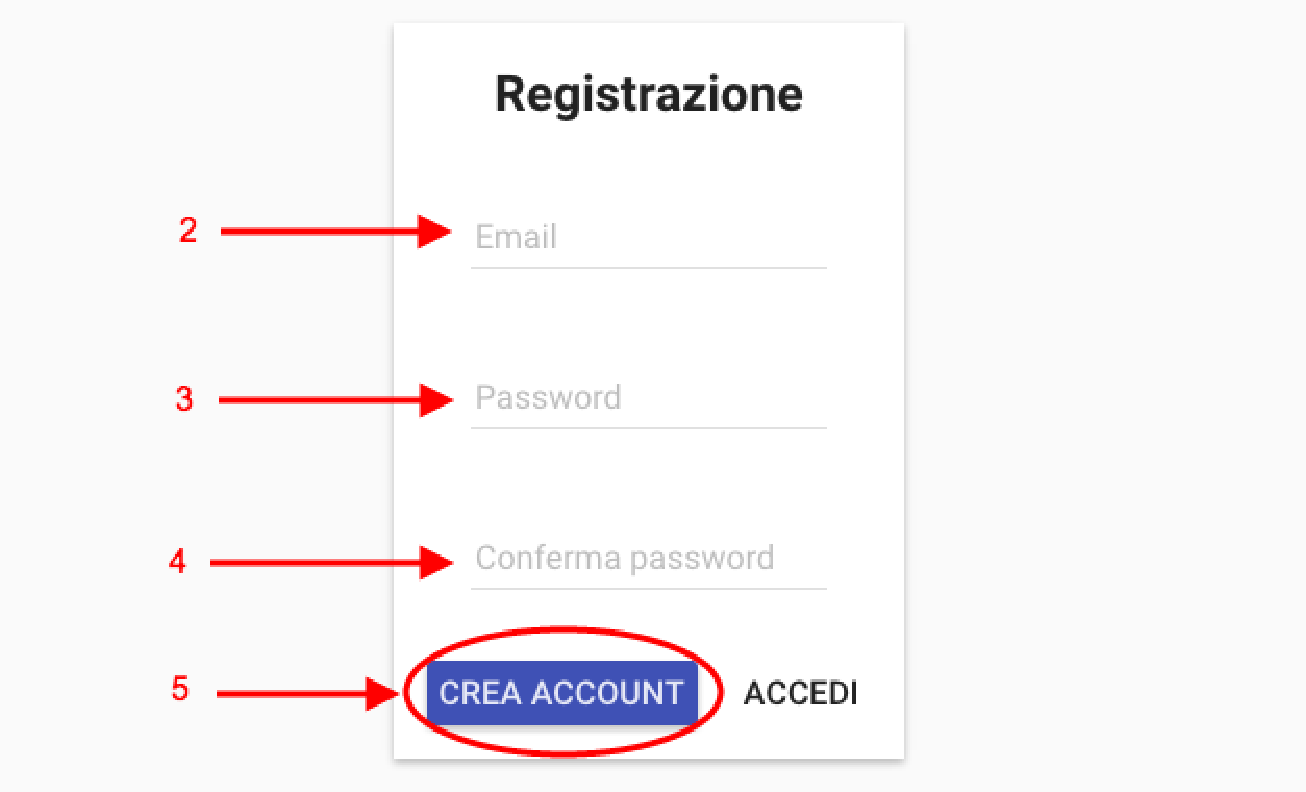
\includegraphics[scale=0.5]{immagini/imgRegistrazione.pdf}
\caption{Form di registrazione}
\end{figure}
%<img src="img/imgRegistrazione.png" alt="imgRegistrazione" width="490" height="440">
Se i dati inseriti non sono corretti o se i campi obbligatori non sono stati compilati verrà visualizzato un messaggio d'errore.
\subsection{Autenticazione}
L'autenticazione permette all'utente di accedere all'applicazione \Premi e di usufruire delle sue funzionalità.\\ Per poter eseguire la procedura di autenticazione l'utente deve aver già effettuato la registrazione al sistema.\\
Per autenticarsi l'utente deve:
\begin{enumerate}
\item Inserire l'indirizzo e-mail utilizzato in fase di registrazione;
\item Inserire la password utilizzata in fase di registrazione;
\item Premere il pulsante \textbf{\textit{Accedi}} per confermare i dati ed accedere al sistema.
\end{enumerate}
\begin{figure}[H]
\centering
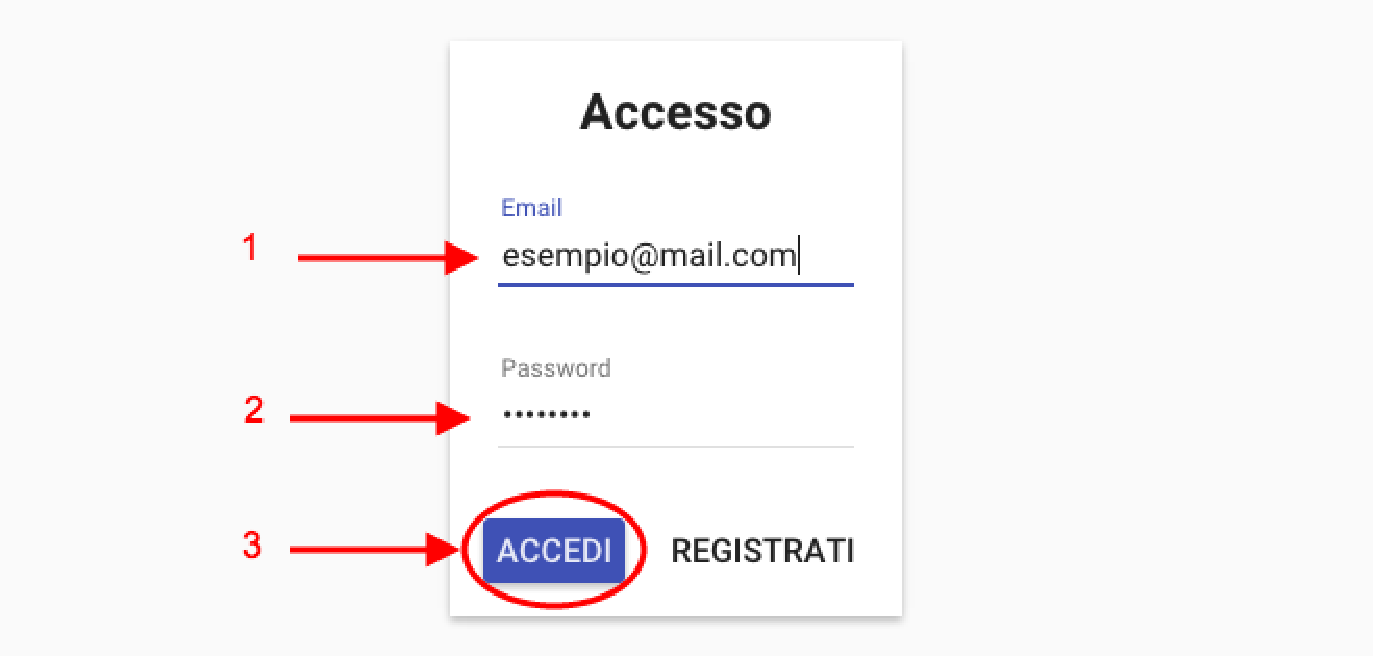
\includegraphics[scale=0.5]{immagini/imgAccesso.pdf}
\caption{Form di accesso}
\end{figure}
%<img src="img/imgAccesso.png" alt="imgAccesso" width="486" height="375">
Se i dati inseriti non sono corretti o se i campi obbligatori non sono stati compilati verrà visualizzato un messaggio d'errore.
\subsection{Uscita}
L'utente può deautenticarsi dal sistema in ogni momento eseguendo la procedura di \textit{Logout}.\\Per effettuare questa procedura l'utente deve trovarsi nella \textit{Dashboard} e premere il pulsante \textbf{\textit{Esci}} presente nella barra di intestazione dell'applicazione .\\
Una volta effettuata la deautenticazione l'utente verrà reindirizzato alla pagina d'accesso dell'applicazione.
\begin{figure}[H]
\centering

\includegraphics[scale=0.3]{immagini/imgEsci.pdf}
\caption{Pulsante di uscita}
\end{figure}
%<img class="imgLunga" src="img/imgEsci.png" alt="imgEsci" width="1276" height="122">
L'utente può accedere alla \textit{Dashboard} sia dalle pagine dedicate alla modifica del \gloxy{progetto}, sia dalla pagina di presentazione tramite il pulsante \textbf{\textit{Chiudi progetto}} presente all'interno del menu della pagina.

\section{Dashboard} \label{dash}
\begin{figure}[H]
\centering
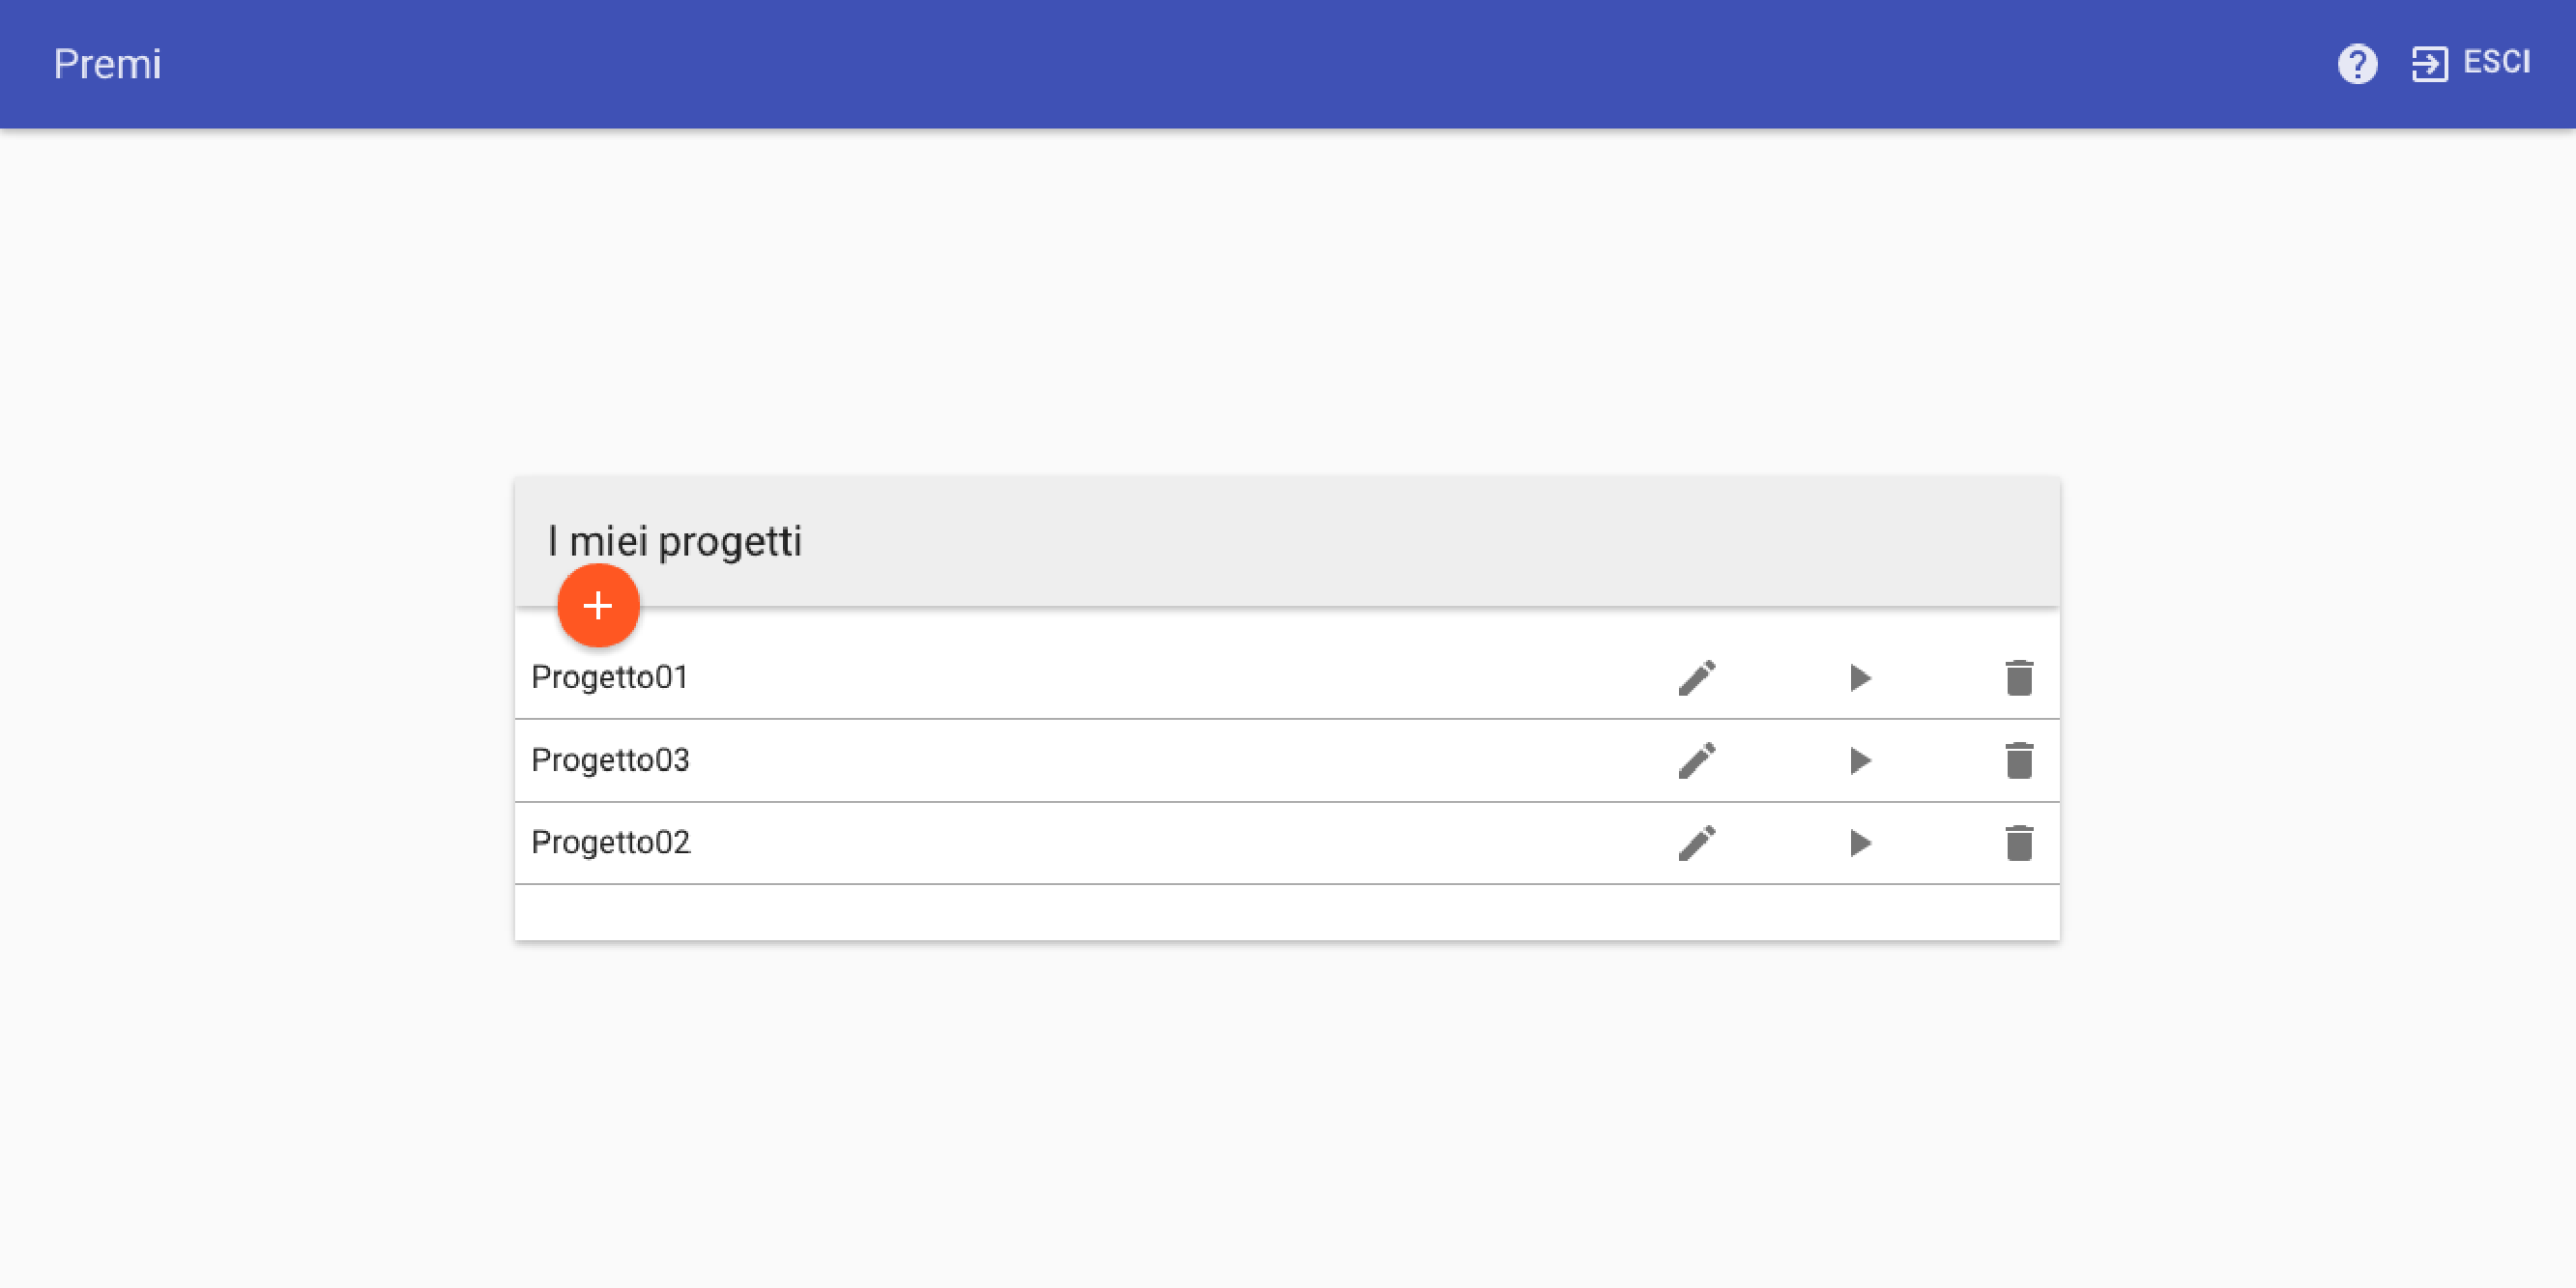
\includegraphics[scale=0.3]{immagini/dashboard.pdf}
\caption{Dashboard}
\end{figure}
In seguito all'autenticazione o alla registrazione l'utente verrà reindirizzato alla \textit{Dashboard}.\\
La \textit{Dashboard} presenta una finestra che contiene al suo interno la lista dei \gloxy{progetti} personali dell'utente. Per ogni \gloxy{progetto}, all'interno della lista, sono presenti dei pulsanti che permettono di eseguite varie azioni sul rispettivo \gloxy{progetto}.
Mediante i pulsanti presenti nella lista dei \gloxy{progetti} l'utente può crearne di nuovi, eliminare dei \gloxy{progetti} già esistenti oppure può modificare o effettuare una presentazione di un determinato \gloxy{progetto}. \\
\begin{figure}[H]
\centering
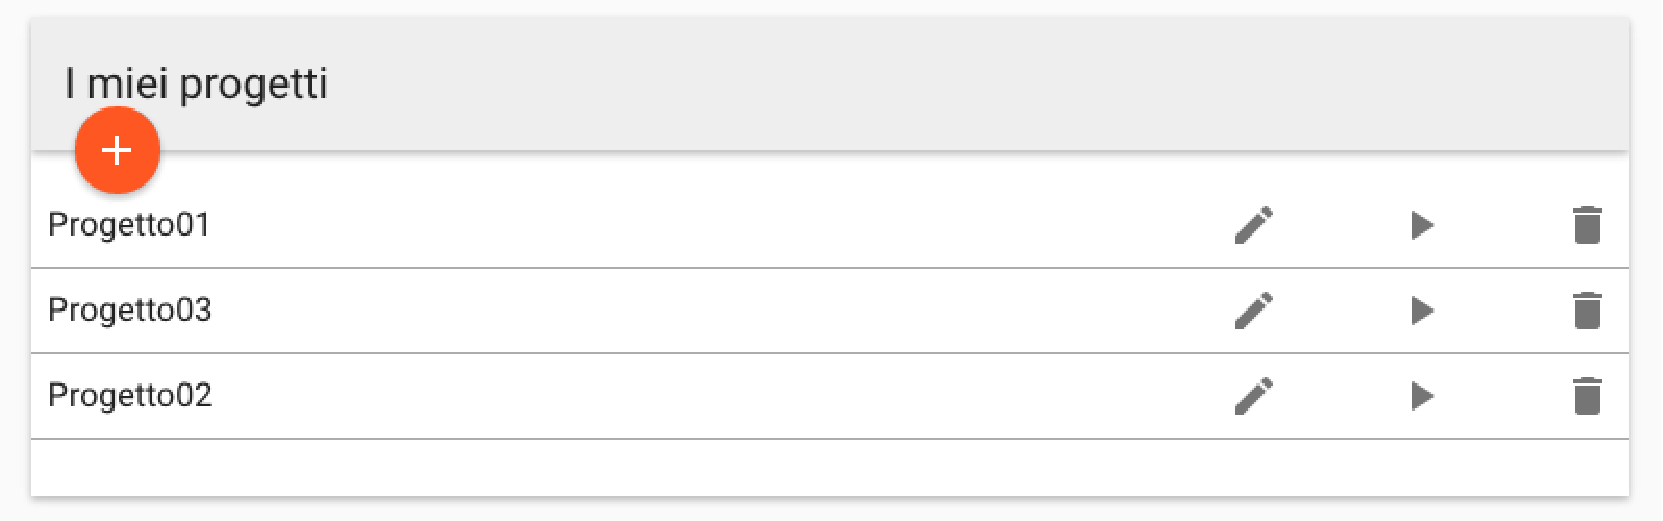
\includegraphics[scale=0.5]{immagini/dashboardVuota.pdf}
\caption{Dashboard - lista dei progetti}
\end{figure}
\subsection{Creazione nuovo progetto}
L'utente può creare un nuovo progetto premendo il pulsante \textbf{più} 
\includegraphics[scale=0.5]{immagini/piuButton.pdf} che si trova nella parte alta della finestra contenente la lista progetti.\\
Effettuando questa azione verrà aggiunto il nuovo progetto alla lista progetti.
\begin{figure}[H]
\centering
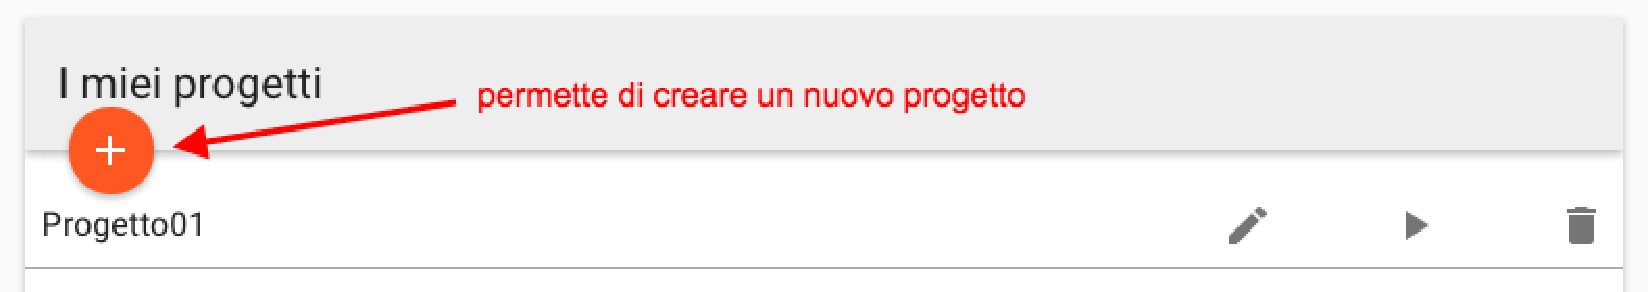
\includegraphics[scale=0.5]{immagini/imgCreaProg.pdf}
\caption{Dashboard - crea nuovo progetto}
\end{figure}
\subsection{Eliminazione di un progetto}
Per poter eliminare un progetto l'utente dovrà premere il pulsante contenente l'icona rappresentante un cestino, che si trova nella riga relativa al progetto che desidera eliminare e confermare l'operazione.
\begin{figure}[H]
\centering
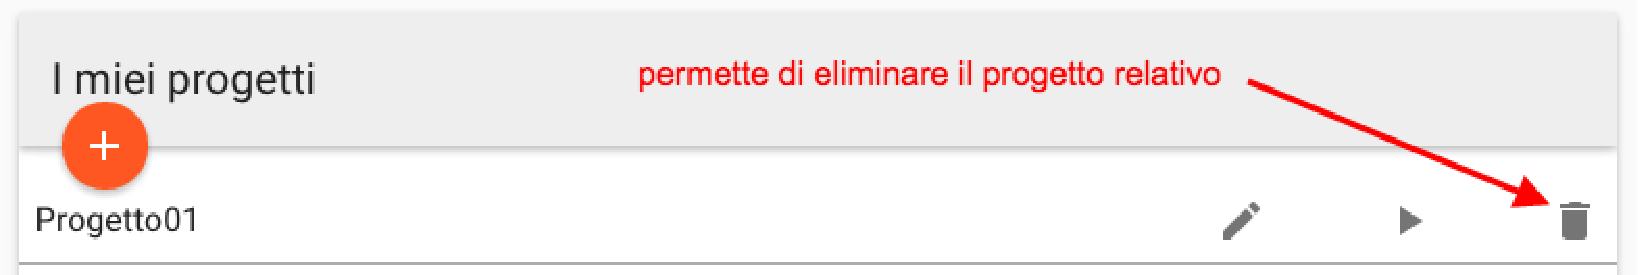
\includegraphics[scale=0.5]{immagini/imgEliminaProg.pdf}
\caption{Dashboard - elimina progetto}
\end{figure}
\subsection{Modificare un progetto}
Per poter accedere alla modalità di editing del progetto l'utente dovrà premere il pulsante contenente l'icona rappresentante una matita, che si trova nella riga relativa al progetto che si desidera modificare.
\begin{figure}[H]
\centering
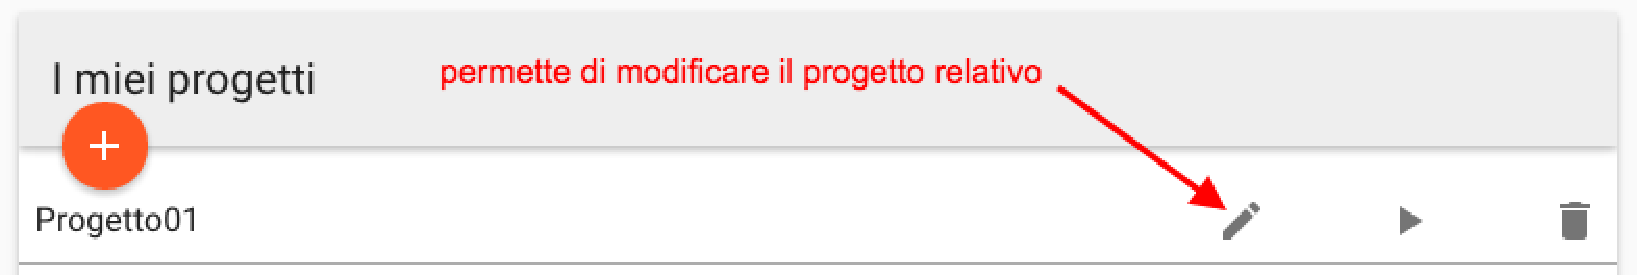
\includegraphics[scale=0.5]{immagini/imgModificaProg.pdf}
\caption{Dashboard - modifica progetto}
\end{figure}
\subsection{Avviare la presentazione di un progetto}
Per poter avviare la presentazione di un \gloxy{progetto}, l'utente deve premere il pulsante contenente l'icona rappresentante il simbolo \textit{play}, che si trova nella riga relativa al \gloxy{progetto} che si desidera presentare.\\ Successivamente, verrà visualizzata una nuova finestra nella quale l'utente dovrà selezionare il \gloxy{percorso} di presentazione e, una volta selezionato, verrà avviata la presentazione.
\begin{figure}[H]
\centering

\includegraphics[scale=0.5]{immagini/imgPresentProg.pdf}
\caption{Dashboard - avviare la presentazione di un progetto}
\end{figure}

\section{Modifica di un progetto} \label{editor}
La pagina per la modifica di un \gloxy{progetto} permette all'utente di creare e modificare la \gloxy{mappa mentale} che sta alla base della presentazione e di definire vari \gloxy{percorsi di presentazione} ad essa associati che descrivono l'ordine in cui i contenuti dei nodi dovranno essere visualizzati durante la presentazione.\\
Al caricamento della pagina l'utente troverà il grafo che rappresenta la mappa mentale.\\
I nodi del grafo possono contenere vari elementi, sia testuali che grafici, che verranno utilizzati per la creazione dei \gloxy{frame} di presentazione.\\
Questi nodi sono collegati fra loro da relazioni gerarchiche (associazioni di tipo padre-figlio) e associazioni logiche, associazioni create dall'utente che mettono in evidenza il collegamento concettuale presente tra due nodi. \\
L'utente troverà nella pagina tutti gli strumenti necessari per poter creare la propria mappa mentale, definire associazioni logiche fra nodi e definire \gloxy{percorsi di presentazione} relativi alla mappa creata.\\
La pagina è formato da due viste, che sono \textit{Modifica mappa} e \textit{Modifica \gloxy{percorsi}}.
Queste due viste permettono di usufruire rispettivamente degli strumenti per la modifica della \gloxy{mappa mentale} e degli strumenti per modifica \gloxy{percorsi} dei \gloxy{percorsi}.\\
L'utente può passare da una vista all'altra tramite i pulsanti \textbf{\textit{Mappa}} e \textbf{\gloxy{Percorsi}} presenti al centro della barra di intestazione dell'applicazione.\\
La barra di intestazione contiene anche altri pulsanti che permettono di modificare la visualizzazione della \gloxy{mappa mentale} e di modificare le impostazioni del \gloxy{progetto}.
\begin{figure}[H]
\centering
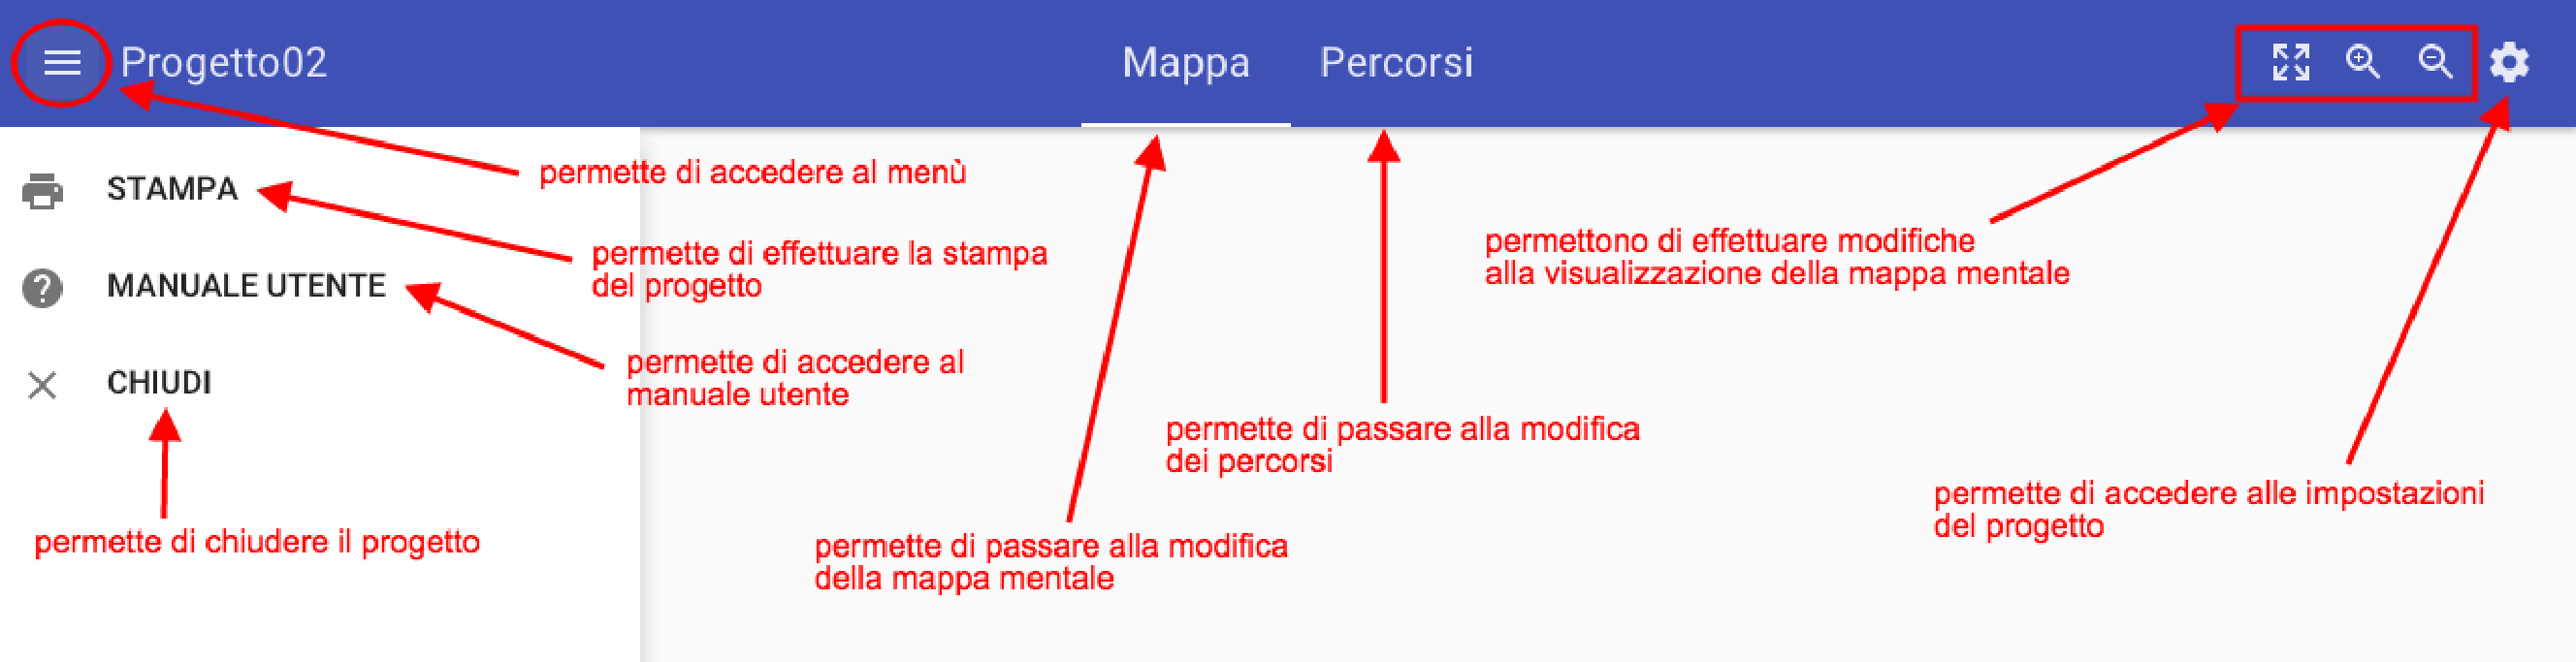
\includegraphics[scale=0.32]{immagini/strumentiHeader.pdf}
\caption{Pulsanti presenti nella barra di intestazione}
\end{figure}
Se il \gloxy{progetto} aperto è appena stato creato, l'utente troverà un nodo già esistente. Questo è il nodo \textit{radice} e rappresenta il nodo base della mappa mentale. L'utente potrà iniziare la creazione della mappa partendo da questo nodo.
\subsection{Modifica della mappa mentale}
\begin{figure}[H]
\centering
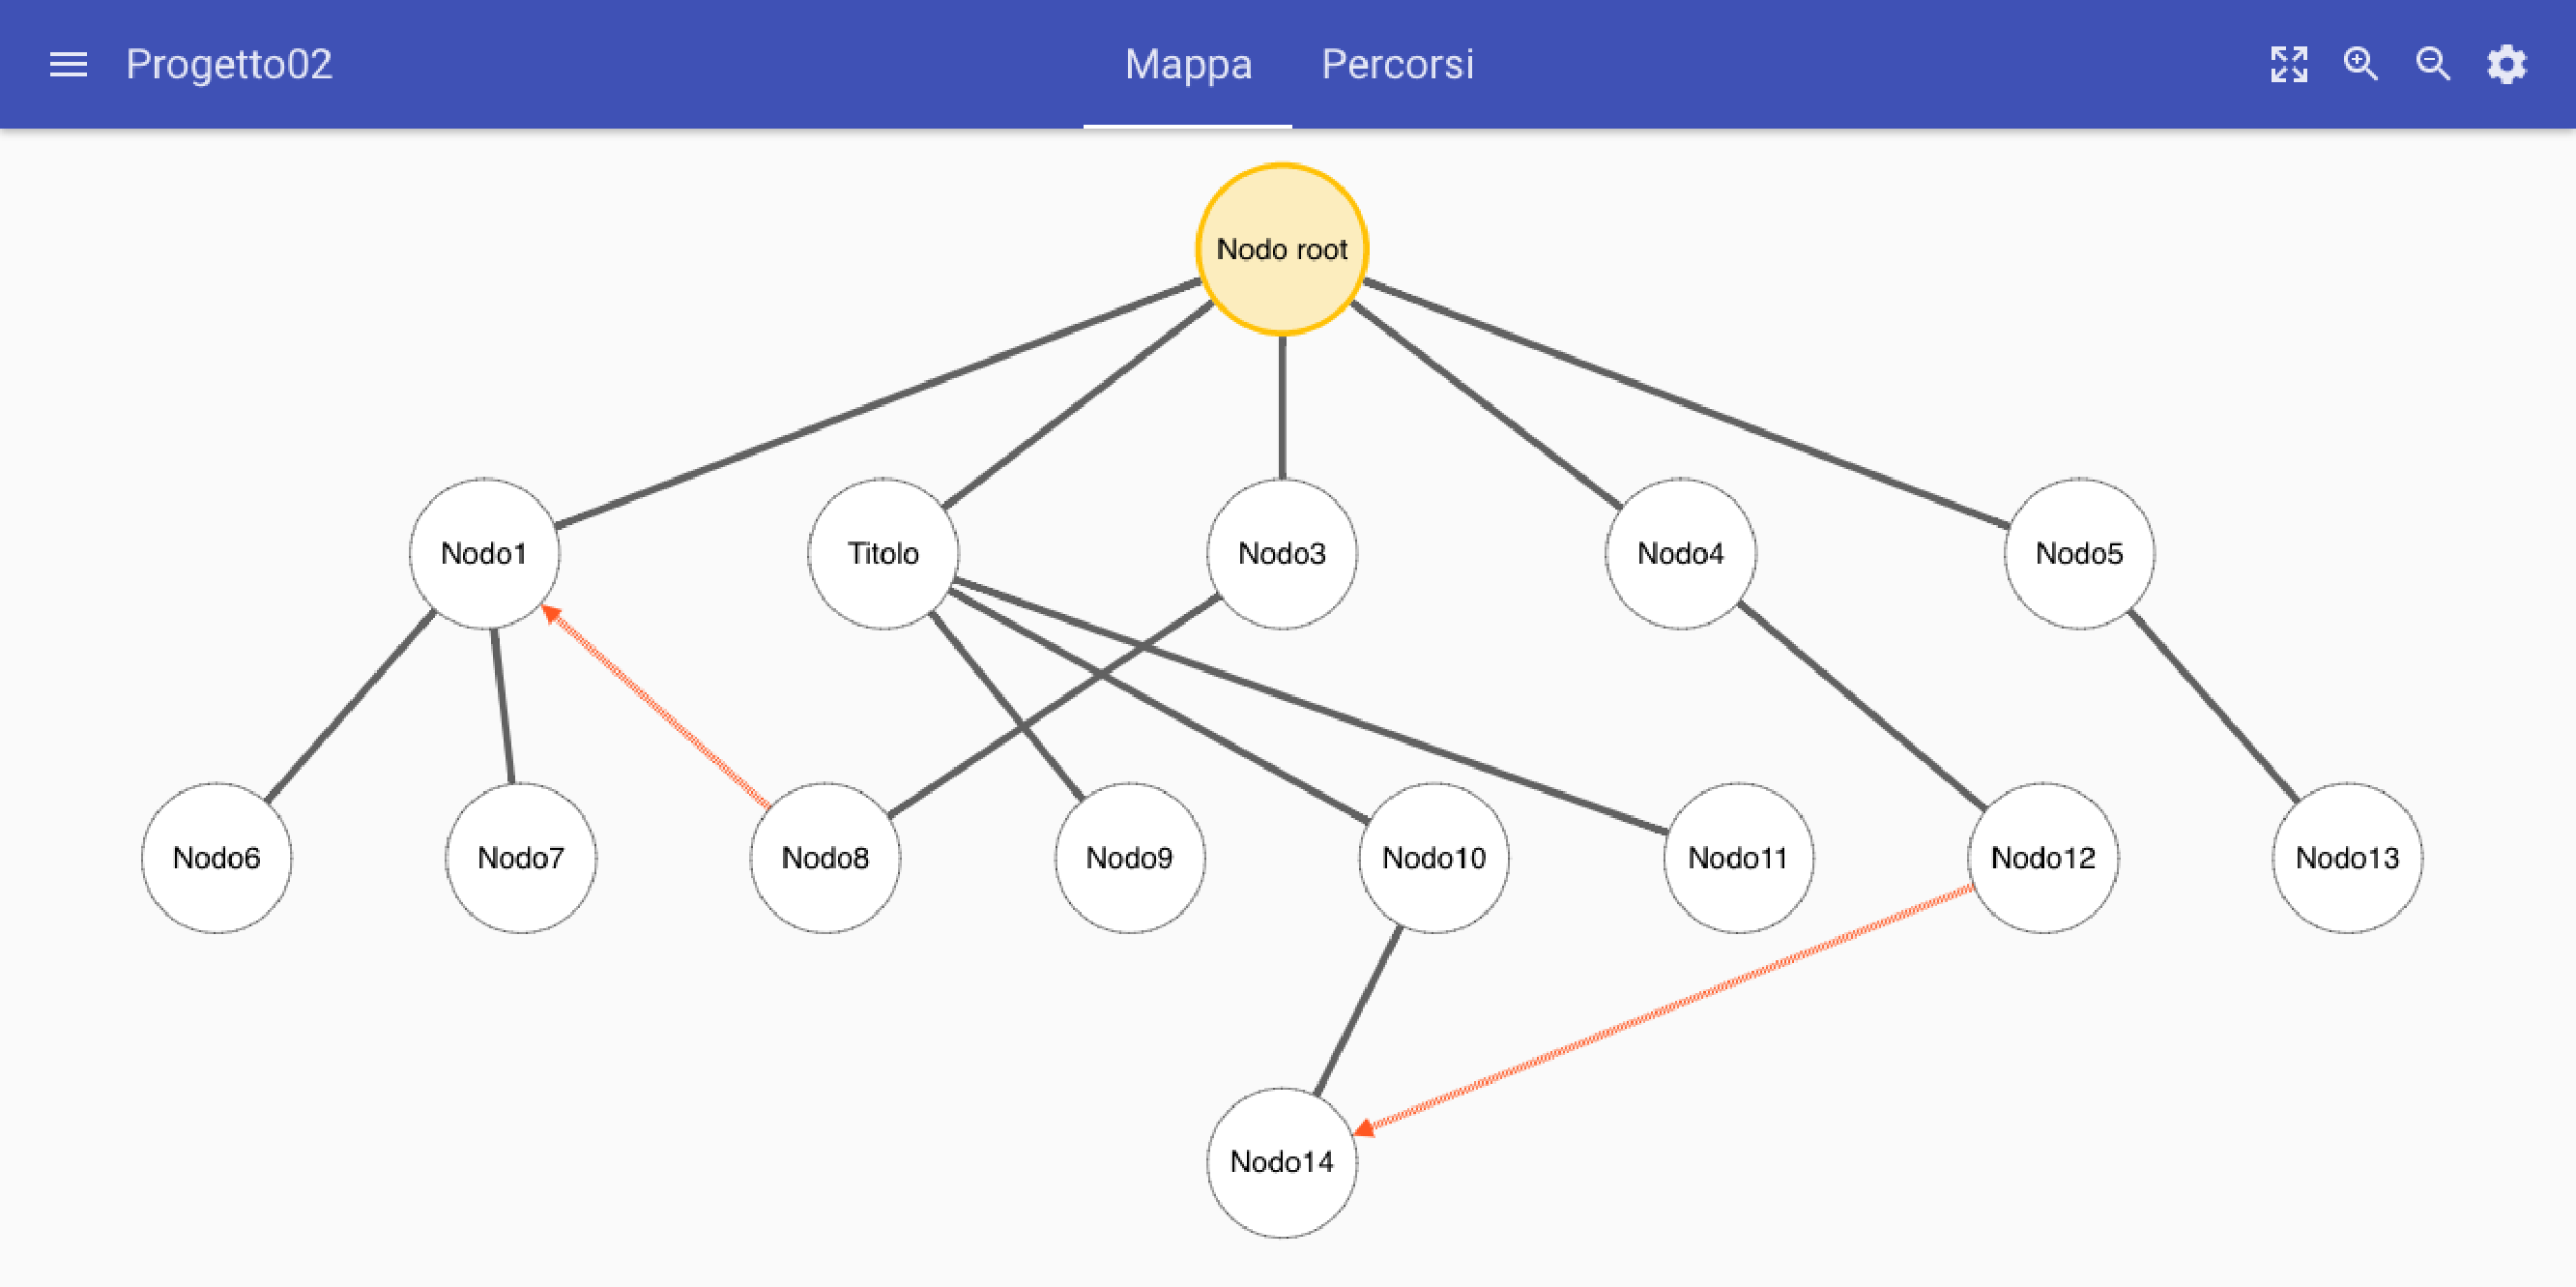
\includegraphics[scale=0.3]{immagini/modificaMappa.pdf}
\caption{Pagina per la modifica della mappa mentale}
\end{figure}
\FloatBarrier
Verranno descritti in seguito gli strumenti che l'utente potrà utilizzare per manipolare la \gloxy{mappa mentale} che desidera creare.

\subsubsection{Spostamento dei nodi}
Per poter spostare un nodo, l'utente deve effettuare il \textit{drag and drop} del nodo nella posizione desiderata. Questa modifica è temporanea dato che la disposizione dei nodi viene calcolata in modo automatico dall'applicazione.

\begin{figure}[H]
\centering
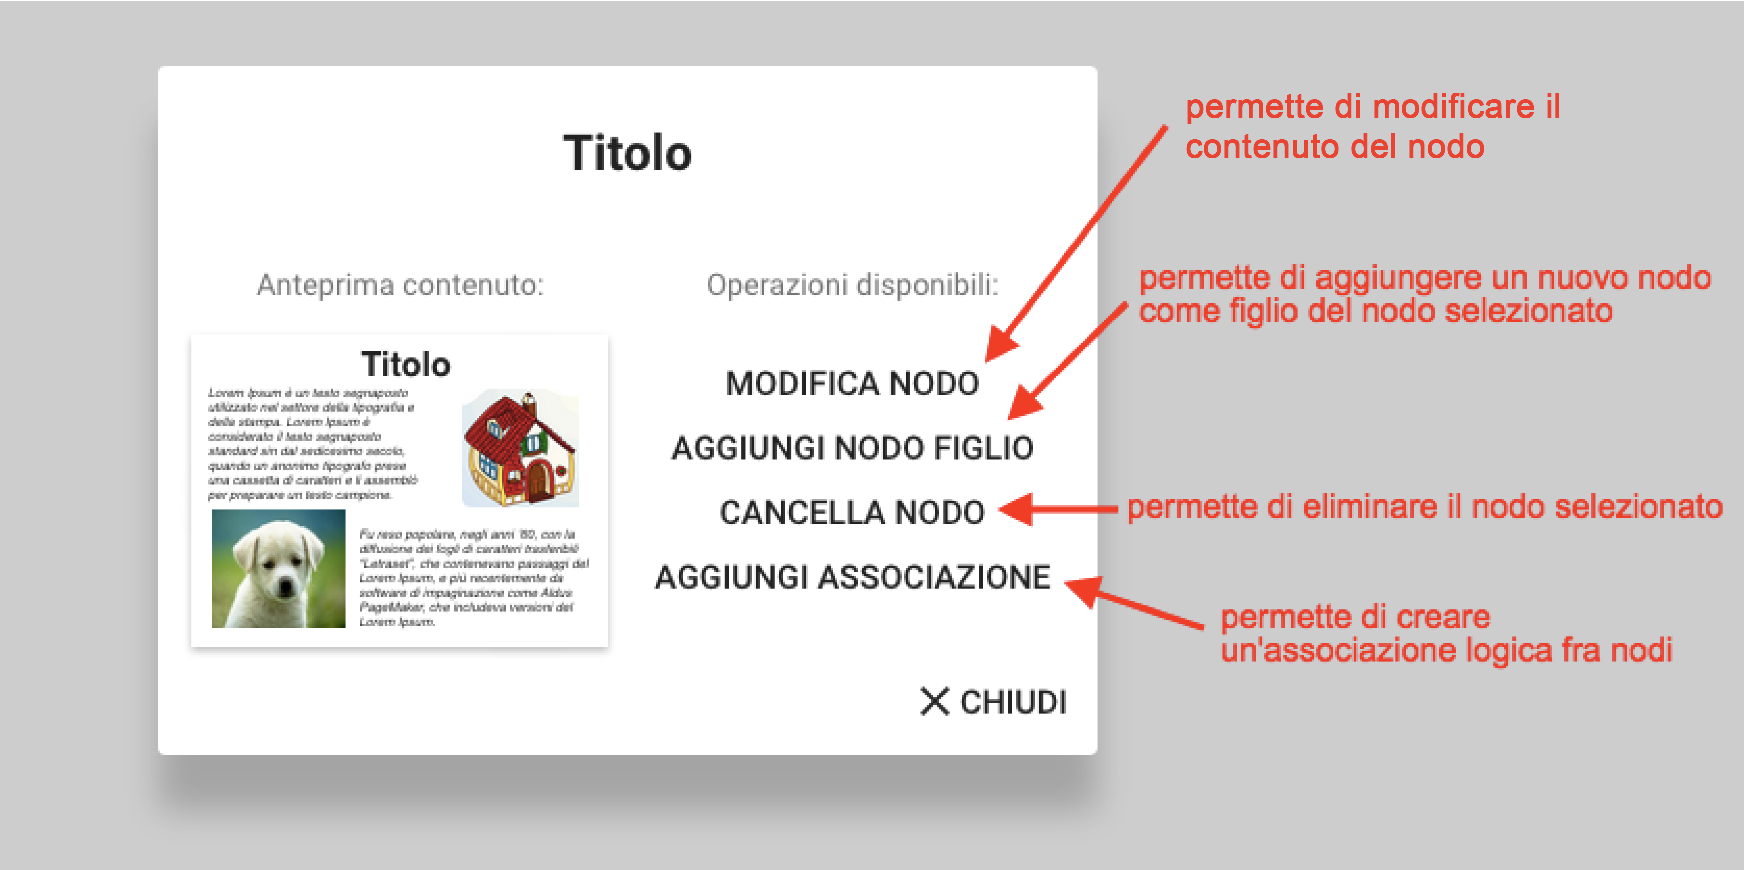
\includegraphics[scale=0.5]{immagini/menuNodoMappa.pdf}
\caption{Menù nodo nella fase di modifica mappa \label{menuNodoMappa}}
\end{figure}
\subsubsection{Creazione nuovo nodo}
Per creare un nuovo nodo, l'utente deve selezionare il nodo a cui desidera aggiungere il nuovo nodo figlio.\\
Verrà visualizzata una nuova finestra contenente un'anteprima dei contenuti del nodo e un elenco delle azioni disponibili. L'utente dovrà selezionare dal menù la voce \textbf{\textit{Aggiungi nodo figlio}}. Una volta premuto il pulsante, il sistema creerà in automatico un nuovo nodo vuoto come figlio del nodo selezionato.
\subsubsection{Eliminazione di un nodo}
Per poter eliminare un nuovo nodo, l'utente deve cliccare sul nodo che desidera eliminare.\\
Verrà visualizzata una nuova finestra contenente un'anteprima dei contenuti del nodo e un elenco delle azioni disponibili. L'utente dovrà selezionare dal menù la voce \textbf{\textit{Cancella nodo}}.\\
Se il nodo che si vuole cancellare ha dei figli o delle associazioni con altri nodi, verranno anchesse cancellate.\\
\subsubsection{Creazione di associazioni logiche}
Per poter creare un'\textit{associazione logica} tra due nodi, l'utente deve:
\begin{enumerate}
\item Selezionare il nodo origine dell'associazione;
\item Selezionare dal menù la voce \textbf{Aggiungi associazione};
\item Dalla finestra che comparirà, selezionare la voce \textbf{seleziona nodo}, per visualizzare la lista dei nodi associabili;
\item Selezionare dalla lista il nodo con cui creare l'associazione;
\item Premere il pulsante di conferma.
\end{enumerate}
L'associazione logica verrà rappresentata tramite una freccia tratteggiata di colore arancio.
\begin{figure}[H]
\centering
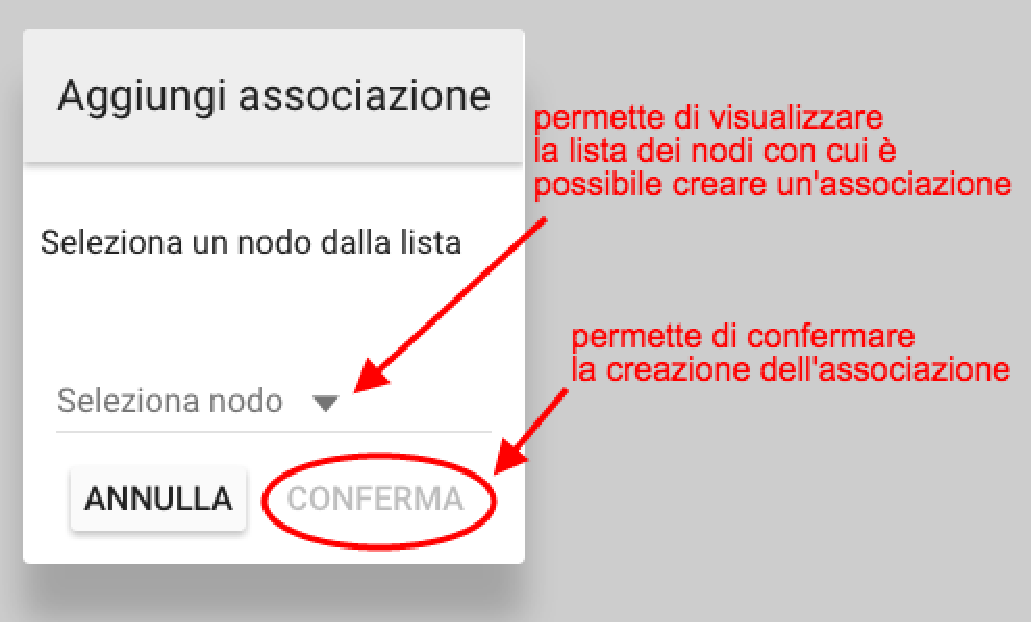
\includegraphics[scale=0.5]{immagini/associazioneMenu.pdf}
\caption{Menù delle associazioni logiche}
\end{figure}
\subsubsection{Eliminazione associazioni logiche}
Per poter eliminare un'\textit{associazione logica}, l'utente deve:
\begin{enumerate}
\item Selezionare l'associazione logica che desidera eliminare;
\item Selezionare la voce \textbf{\textit{cancella associazione}} dal menù che comparirà.
\end{enumerate}
\subsubsection{Inserimento contenuti}
Per poter inserire dei contenuti all'interno di un nodo, l'utente deve selezionare il nodo nel quale desidera inserire dei contenuti.\\
Verrà visualizzata una nuova finestra contenente un'anteprima dei contenuti del nodo e un elenco di azioni possibili. L'utente dovrà selezionare dal menù la voce \textbf{\textit{Modifica nodo}}.\\
Verrà visualizzata una nuova finestra nella quale sarà possibile gestire i contenuti del nodo, le varie funzionalità offerte verranno descritte nella sezione \nameref{editNodo}.
\subsection{Modifica del contenuto di un nodo}\label{editNodo}
In questa sezione verrà spiegato come utilizzare le funzionalità offerte dall'applicazione per gestire i contenuti di un nodo della mappa mentale.\\
La finestra mostra nella parte sinistra due pulsanti, che sono rispettivamente \textbf{\textit{Aggiungi testo}} e \textbf{\textit{Aggiungi immagine}} e, nella parte destra una rappresentazione del \gloxy{frame} con i suoi contenuti.\\
L'utente può selezionare i contenuti \textit{cliccandoci} sopra e vedrà apparire, sotto i pulsanti per l'inserimento di nuovi contenuti, una vista che permette di effettuare le modifiche sull'elemento selezionato.
\begin{figure}[H]
\centering
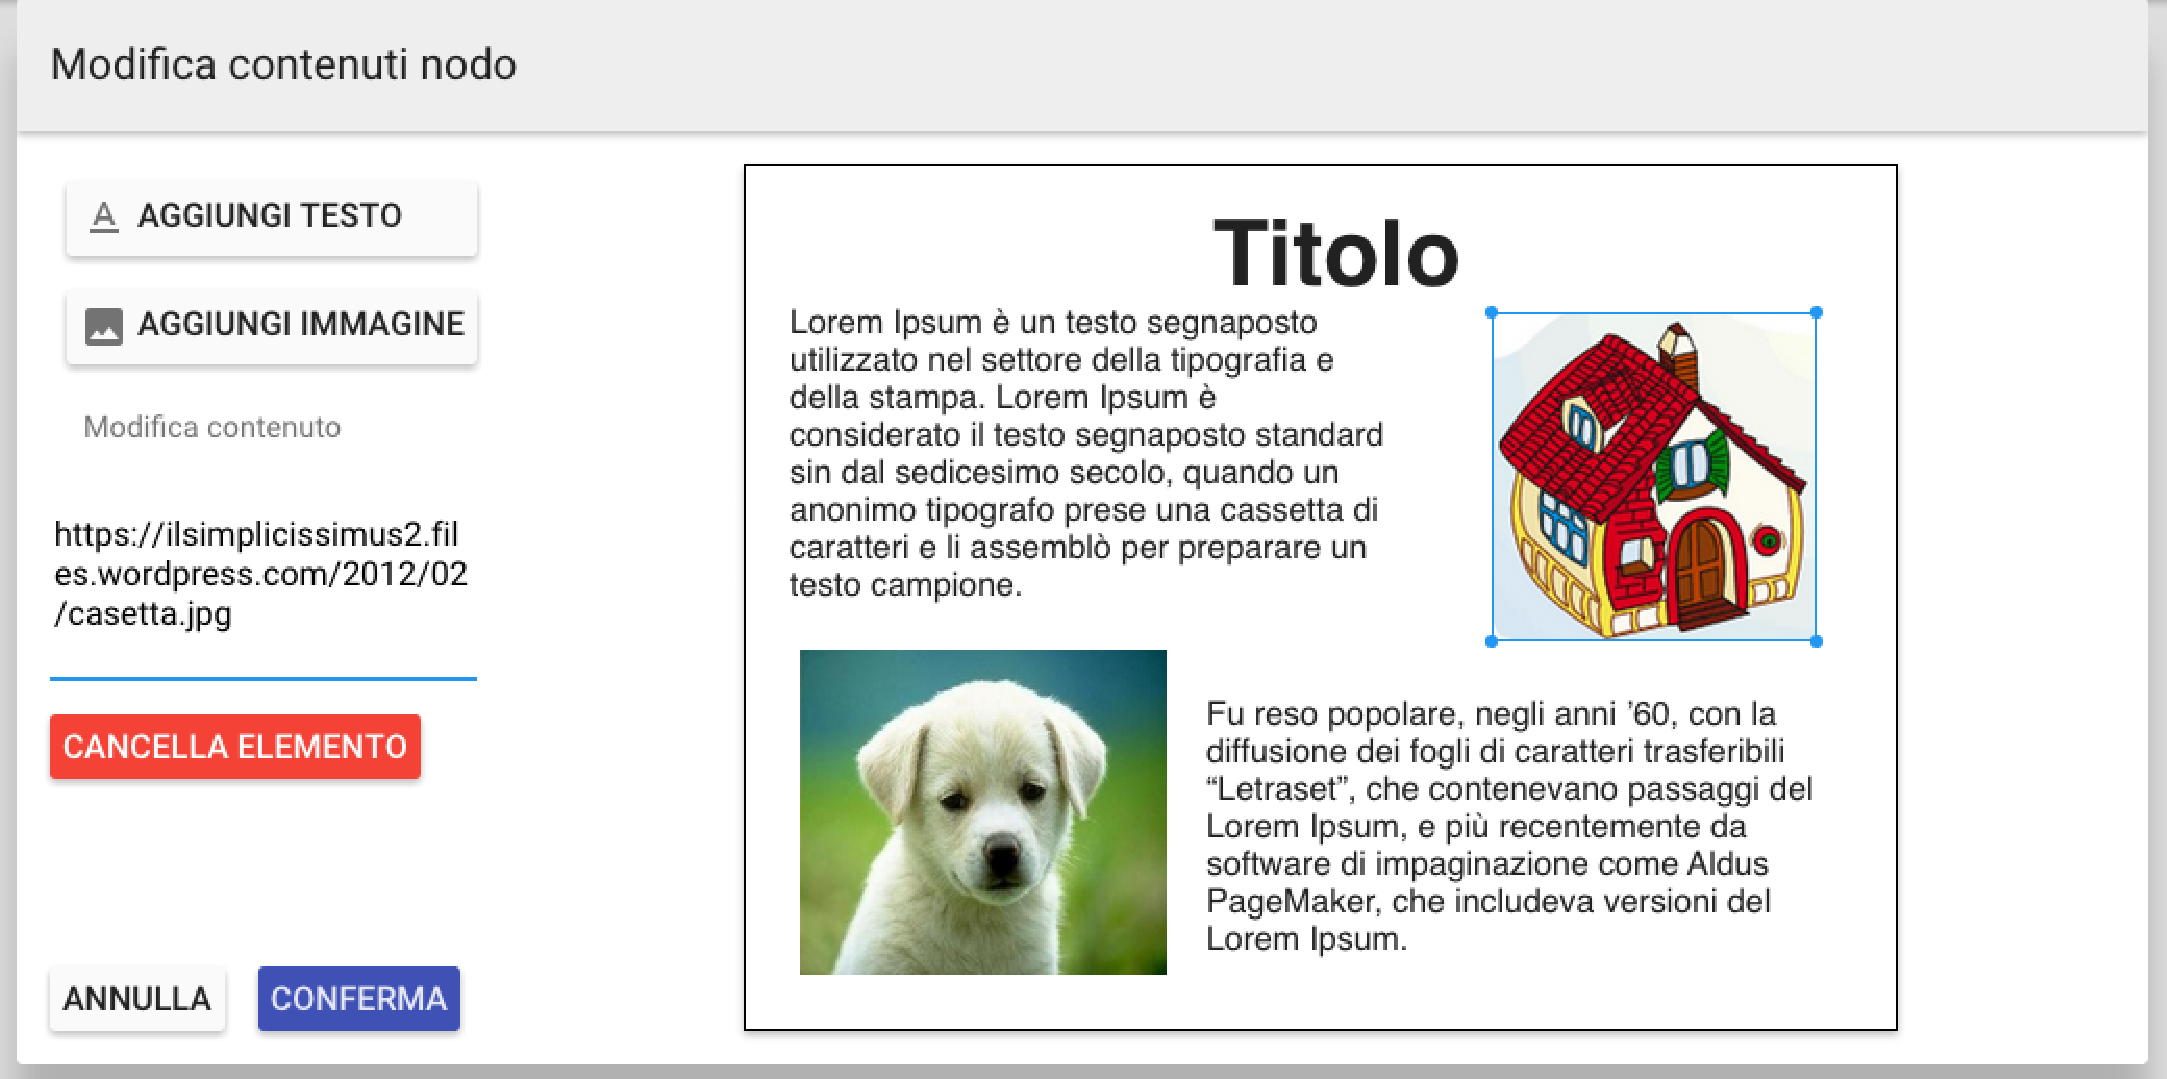
\includegraphics[scale=0.38]{immagini/modificaNodo.pdf}
\caption{Menù di modifica nodo \label{modificaNodo}}
\end{figure}
\subsubsection{Aggiungere del testo}
Per poter inserire del testo all'interno del nodo, l'utente deve premere il pulsante \textbf{\textit{Aggiungi testo}}, in questo modo verrà inserito all'interno del \gloxy{frame} un nuovo \textit{elemento testuale} contenente del testo di \textit{default}.\\
Per modificare il testo l'utente dovrà selezionare il nuovo elemento, in modo da rendere visibile lo strumento di modifica nella parte sinistra della finestra.
\subsubsection{Aggiungere un immagine}
Per poter inserire un'immagine all'interno del nodo, l'utente deve premere il pulsante \textbf{\textit{Aggiungi immagine}}, in questo modo verrà inserita all'interno del \gloxy{frame} un'immagine di default.
Per modificare l'immagine, l'utente dovrà selezionare il nuovo elemento e modificare l'URL in esso contenuto tramite lo strumento di modifica che diventerà visibile nella parte sinistra della finestra, inserendo l'URL della nuova immagine.\\
L'URL dell'immagine deve riferirsi ad un'immagine presente sul \textbf{\gloxy{web}}.
\subsubsection{Posizionamento contenuti}
Per poter posizionare un contenuto all'interno del \gloxy{frame}, l'utente dovrà trascinarlo, tramite \textit{drag and drop}, nella posizione desiderata.
\subsubsection{Ridimensionamento contenuto}
Per poter ridimensionare un contenuto, l'utente dovrà selezionare il contenuto che desidera ridimensionare e posizionandosi sui bordi del contenuto selezionato ridimensionarlo.
\subsection{Modifica dei percorsi di presentazione}
\begin{figure}[H]
\centering
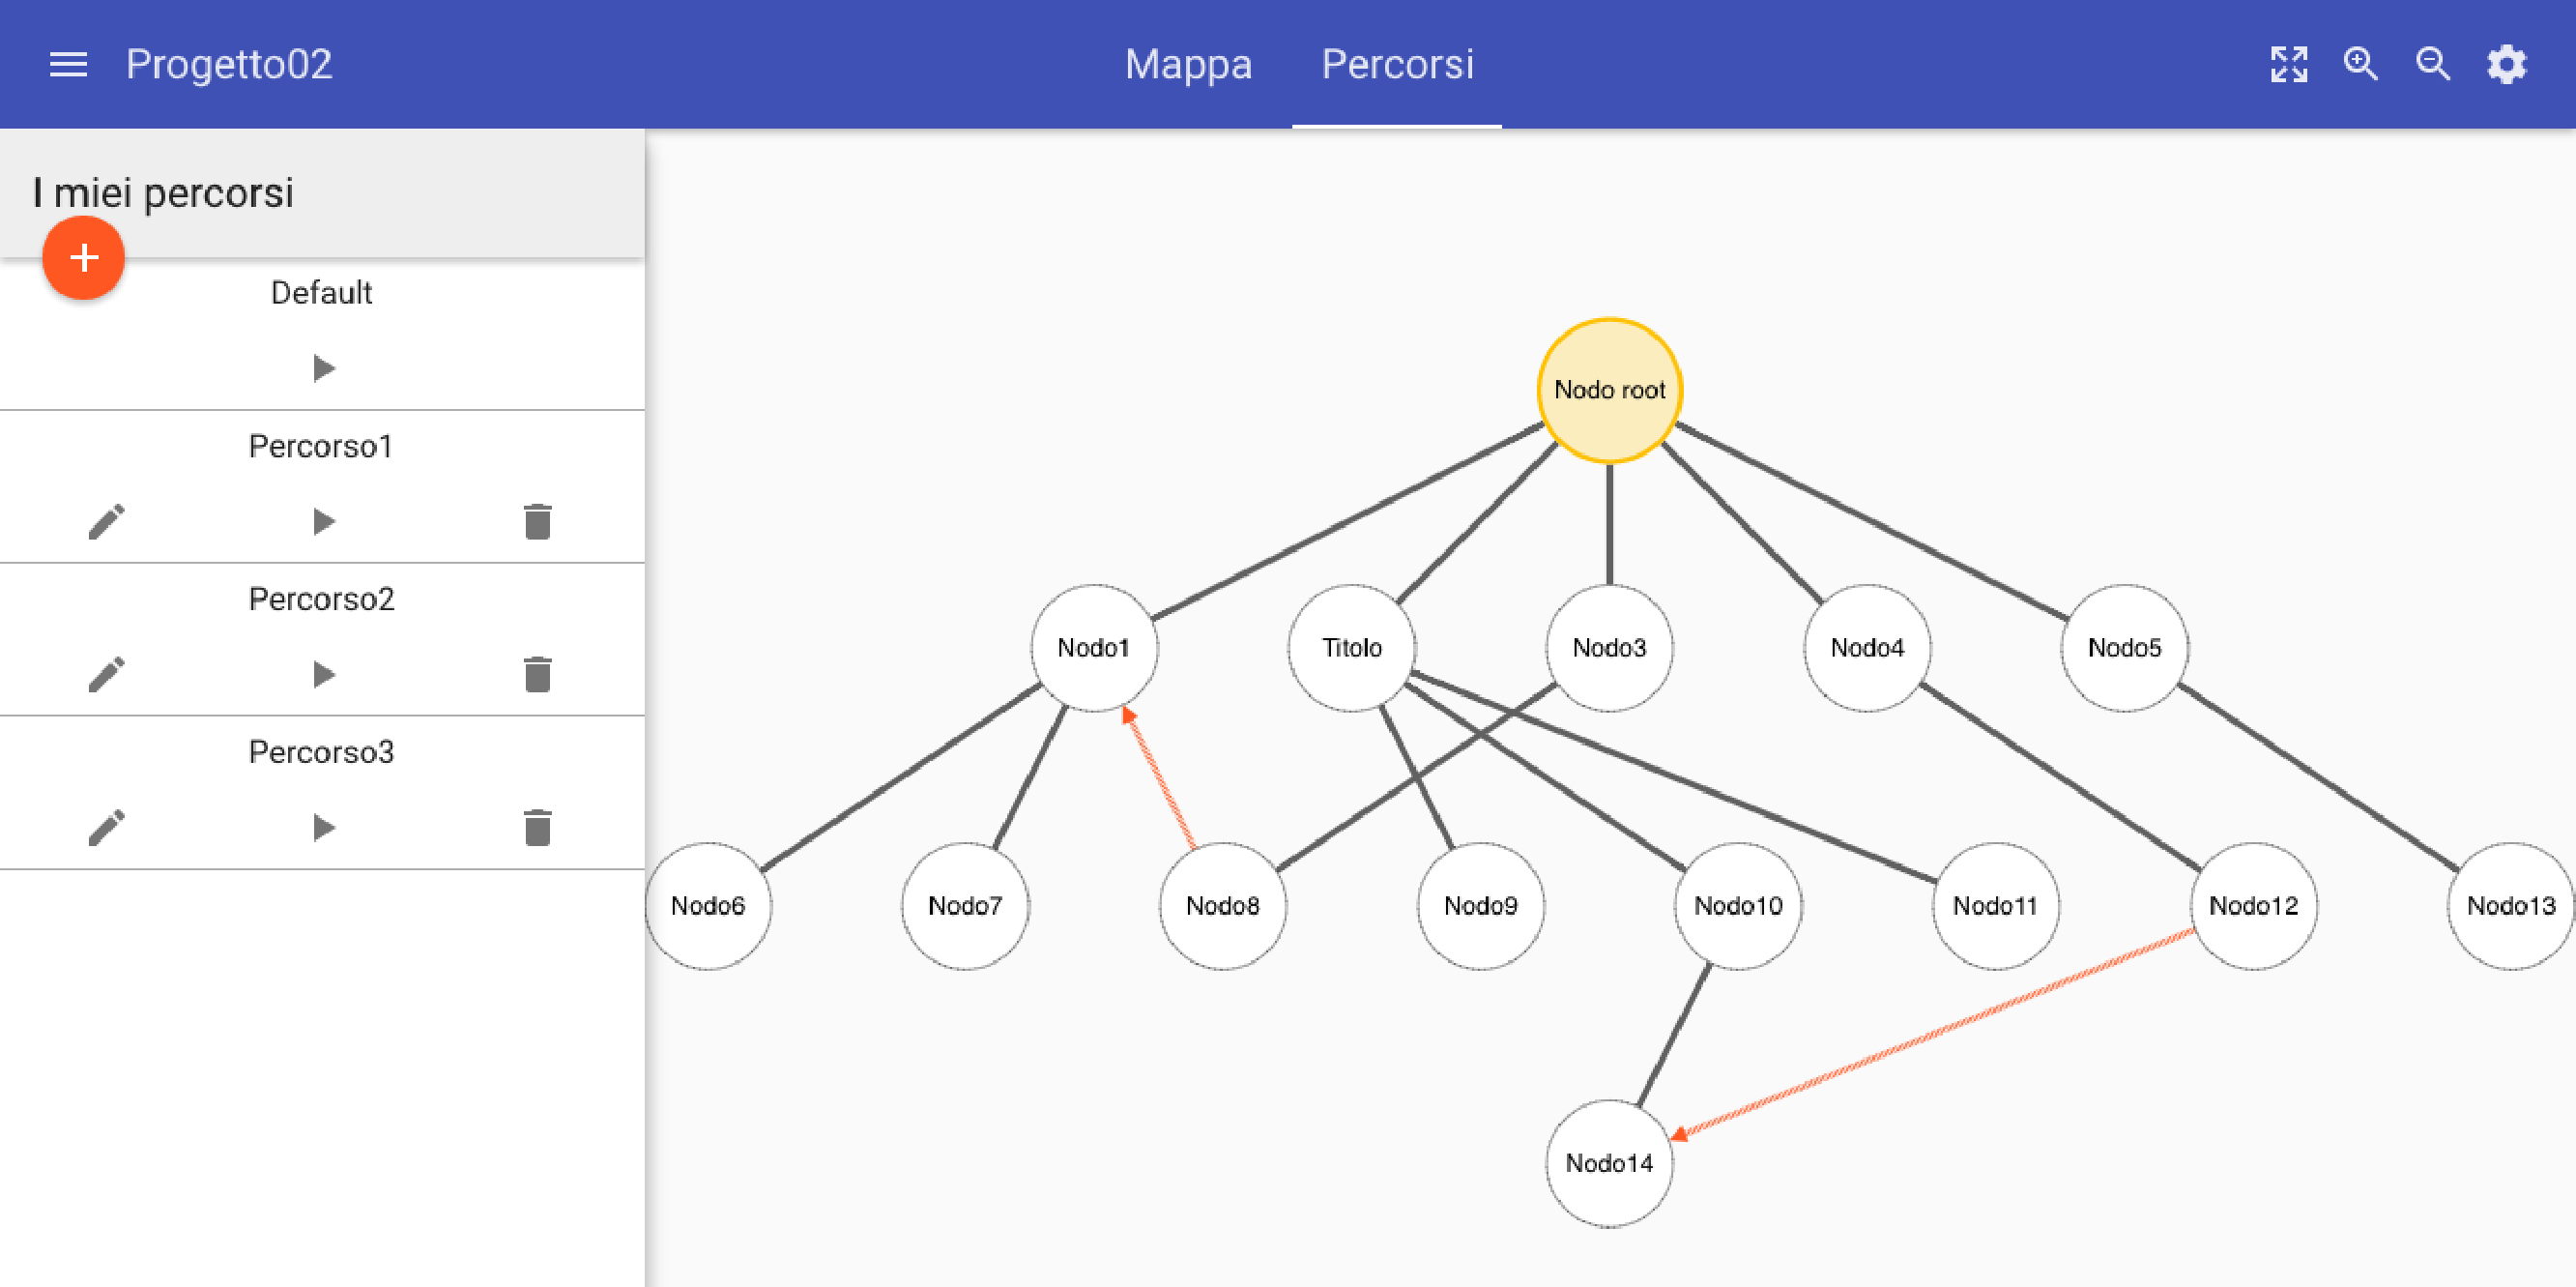
\includegraphics[scale=0.3]{immagini/modificaPercorsi.pdf}
\caption{Pagina per la modifica del percorsi}
\end{figure}
\FloatBarrier
Verranno descritte in seguito gli strumenti che l'utente potrà utilizzare per la creazione e la gestione dei \gloxy{percorsi} personalizzati di presentazione.
\subsubsection{Creazione nuovo percorso}
Per poter creare un nuovo \gloxy{percorso} di presentazione, l'utente deve trovarsi nella vista \textit{\gloxy{percorsi}} e deve premere il pulsante \textbf{più} 
\includegraphics[scale=0.5]{immagini/piuButton.pdf} presente nella parte sinistra della vista.
Verrà visualizzata una finestra, nella quale l'utente dovrà inserire il nome del nuovo \gloxy{percorso} e premere il pulsante \textbf{Aggiungi}.
\subsubsection{Modifica di un percorso}
Per poter modificare il nome di un \gloxy{percorso} ed il suo contenuto, l'utente deve premere il pulsante con l'icona rappresentante una matita presente nella lista \gloxy{percorsi} relativa al \gloxy{percorso} che desidera modificare.\\
Dalla finestra che compare l'utente potrà rinominare il \gloxy{percorso di presentazione} oppure rimuovere dei nodi dal \gloxy{percorso}.\\
Per il \gloxy{percorso} di default non è disponibile questa opzione.
%immagine della schermata
\begin{figure}[H]
\centering
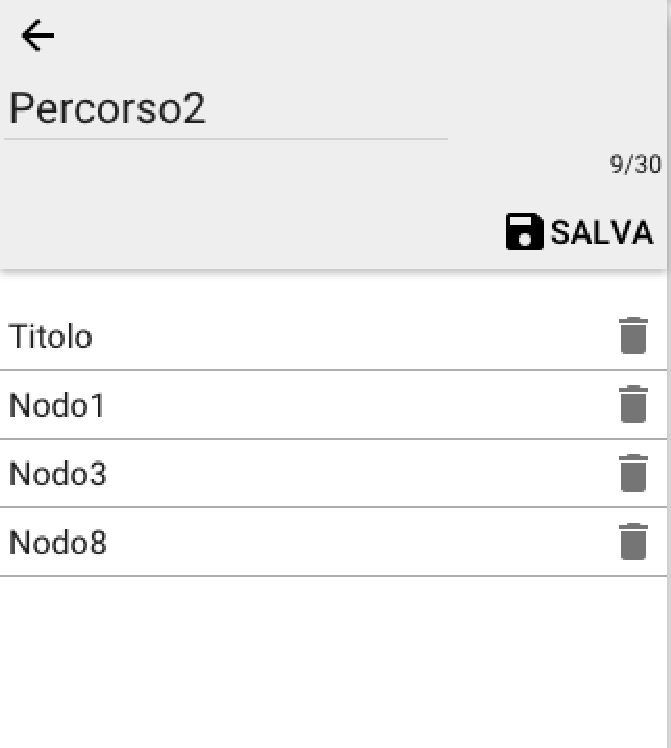
\includegraphics[scale=0.6]{immagini/modificaPercorso.pdf}
\caption{Modifica percorsi - lista dei nodi di un percorso}
\end{figure}
\FloatBarrier
\subsubsection{Eliminazione percorso}
Per poter eliminare un \gloxy{percorso}, l'utente deve premere il pulsante con l'icona rappresentante un cestino presente nella lista \gloxy{percorsi} e relativa al \gloxy{percorso} che desidera eliminare.\\
Per il \gloxy{percorso} di default non è disponibile questa opzione.
\begin{figure}[H]
\centering
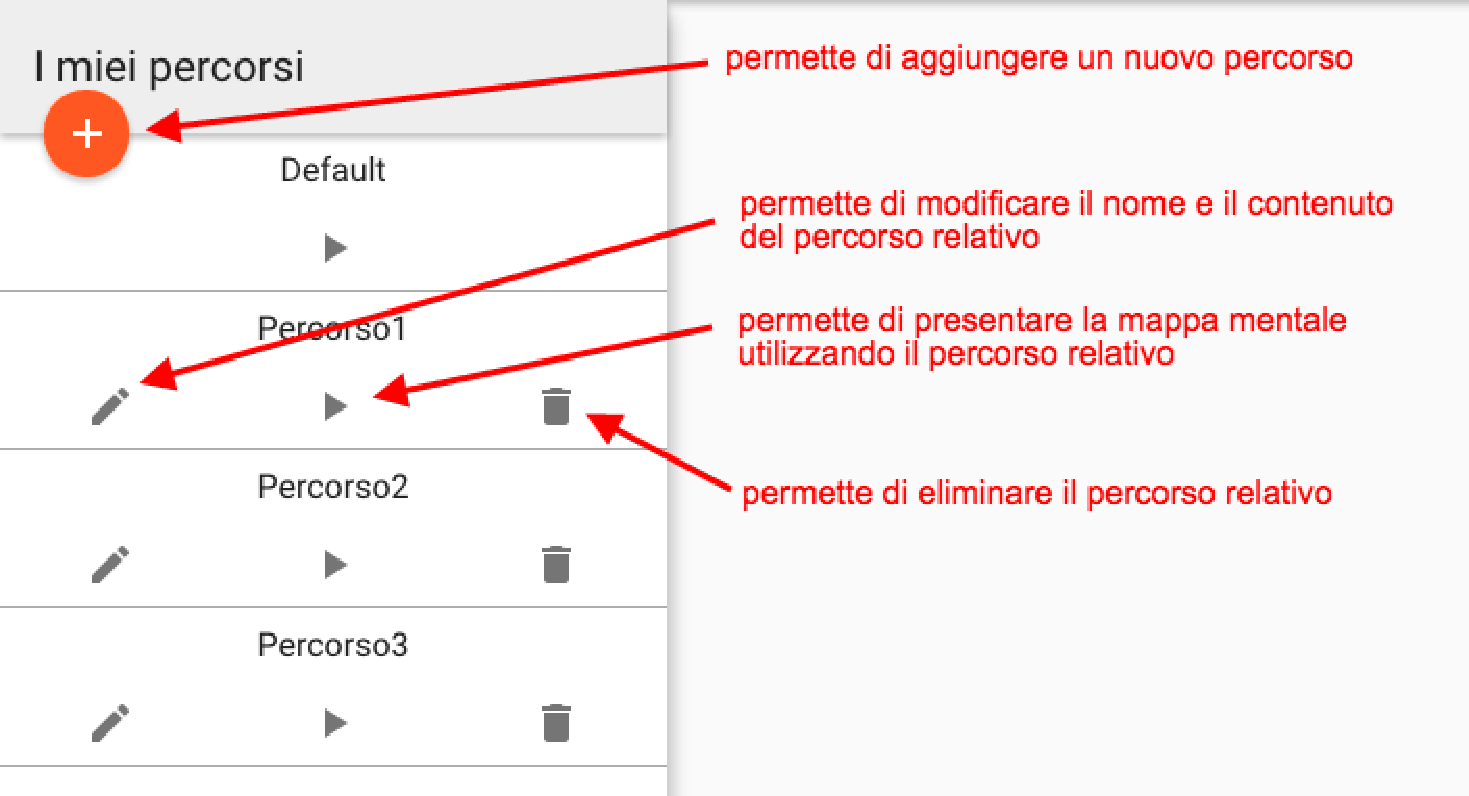
\includegraphics[scale=0.5]{immagini/menuPercorsi.pdf}
\caption{Modifica percorsi - lista dei percorsi}
\end{figure}
\subsubsection{Aggiunta di un nodo ad un percorso di presentazione}
Per poter aggiungere un nodo ad un \gloxy{percorso di presentazione} l'utente deve:
\begin{enumerate}
\item Trovarsi nella vista \textbf{\gloxy{Percorsi}};
\item Selezionare il nodo dalla mappa mentale;
\item Selezionare dalla finestra che comparirà, il \gloxy{percorso} al quale aggiungere il nodo selezionato.
\end{enumerate}
\begin{figure}[H]
\centering
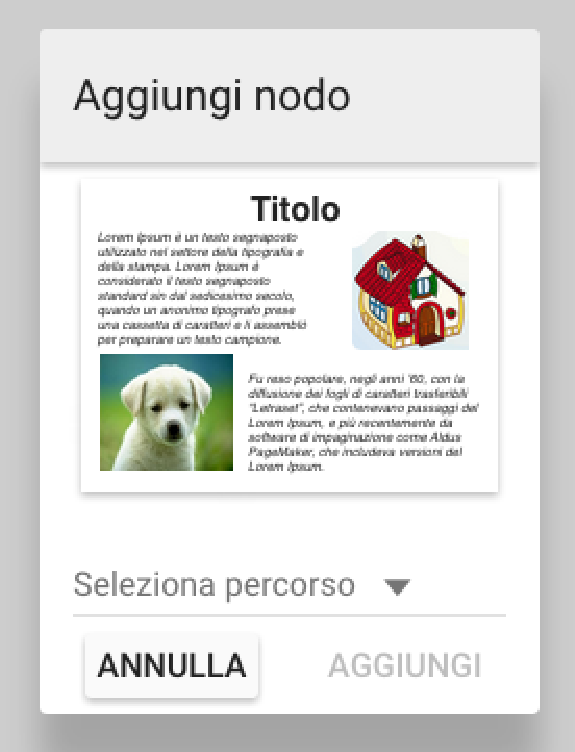
\includegraphics[scale=0.6]{immagini/aggiuntaNodoAPercorso2.pdf}
\caption{Aggiunta di un nodo ad un percorso di presentazione}
\end{figure}
\subsection{Modifica delle impostazioni del progetto}
Tramite questo strumento l'utente può effettuare delle modifiche al \gloxy{progetto} sul quale sta lavorando.\\ In particolare potrà modificare:
\begin{itemize}
\item Il nome del \gloxy{progetto};
\item Il colore di sfondo dei \gloxy{frame} del \gloxy{progetto};
\item Il colore del testo dei \gloxy{frame} del \gloxy{progetto};
\item Il font utilizzato nei \gloxy{frame} del \gloxy{progetto}.
\end{itemize}
La finestra \textbf{\textit{Impostazioni del }\gloxy{progetto}} può essere raggiunta premendo l'icona rappresentante un ingranaggio

\includegraphics[scale=0.5]{immagini/impostazioniButton.pdf}, presente all'interno della barra di intestazione dell'applicazione.
\begin{figure}[H]
\centering
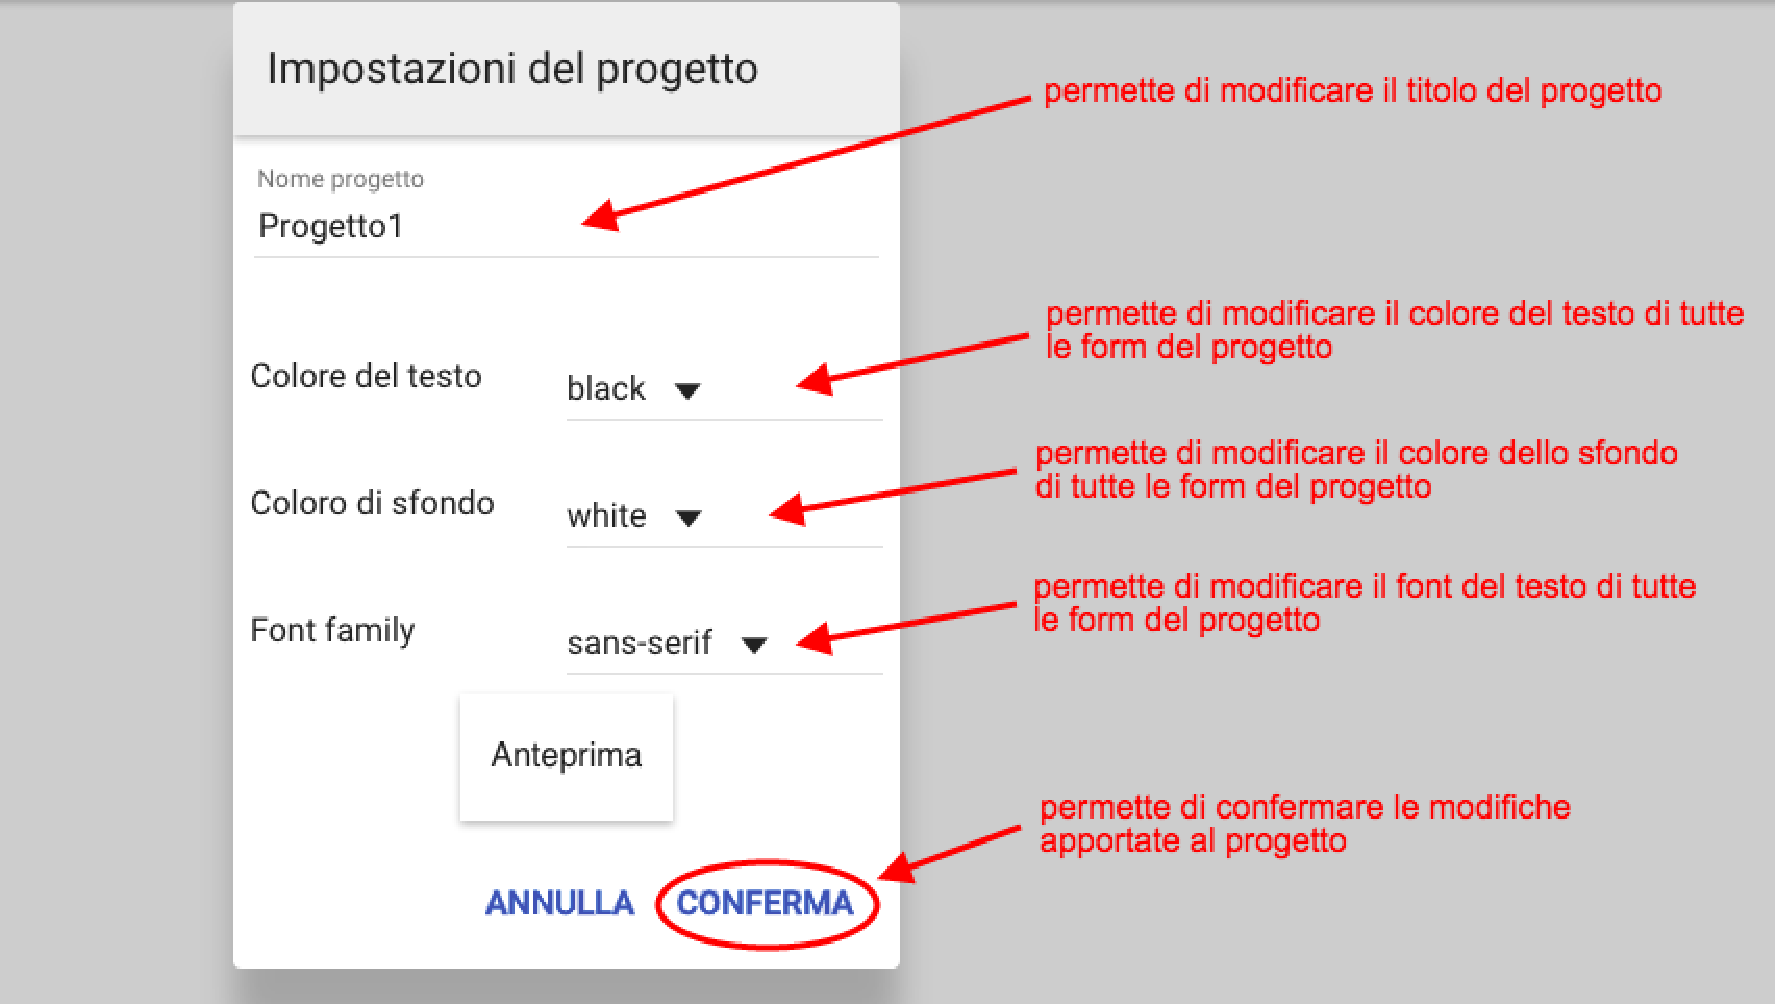
\includegraphics[scale=0.5]{immagini/impostazioneProgetto.pdf}
\caption{Impostazioni del progetto}
\end{figure}

\section{Presentazione} \label{pres}
\begin{figure}[H]
\centering
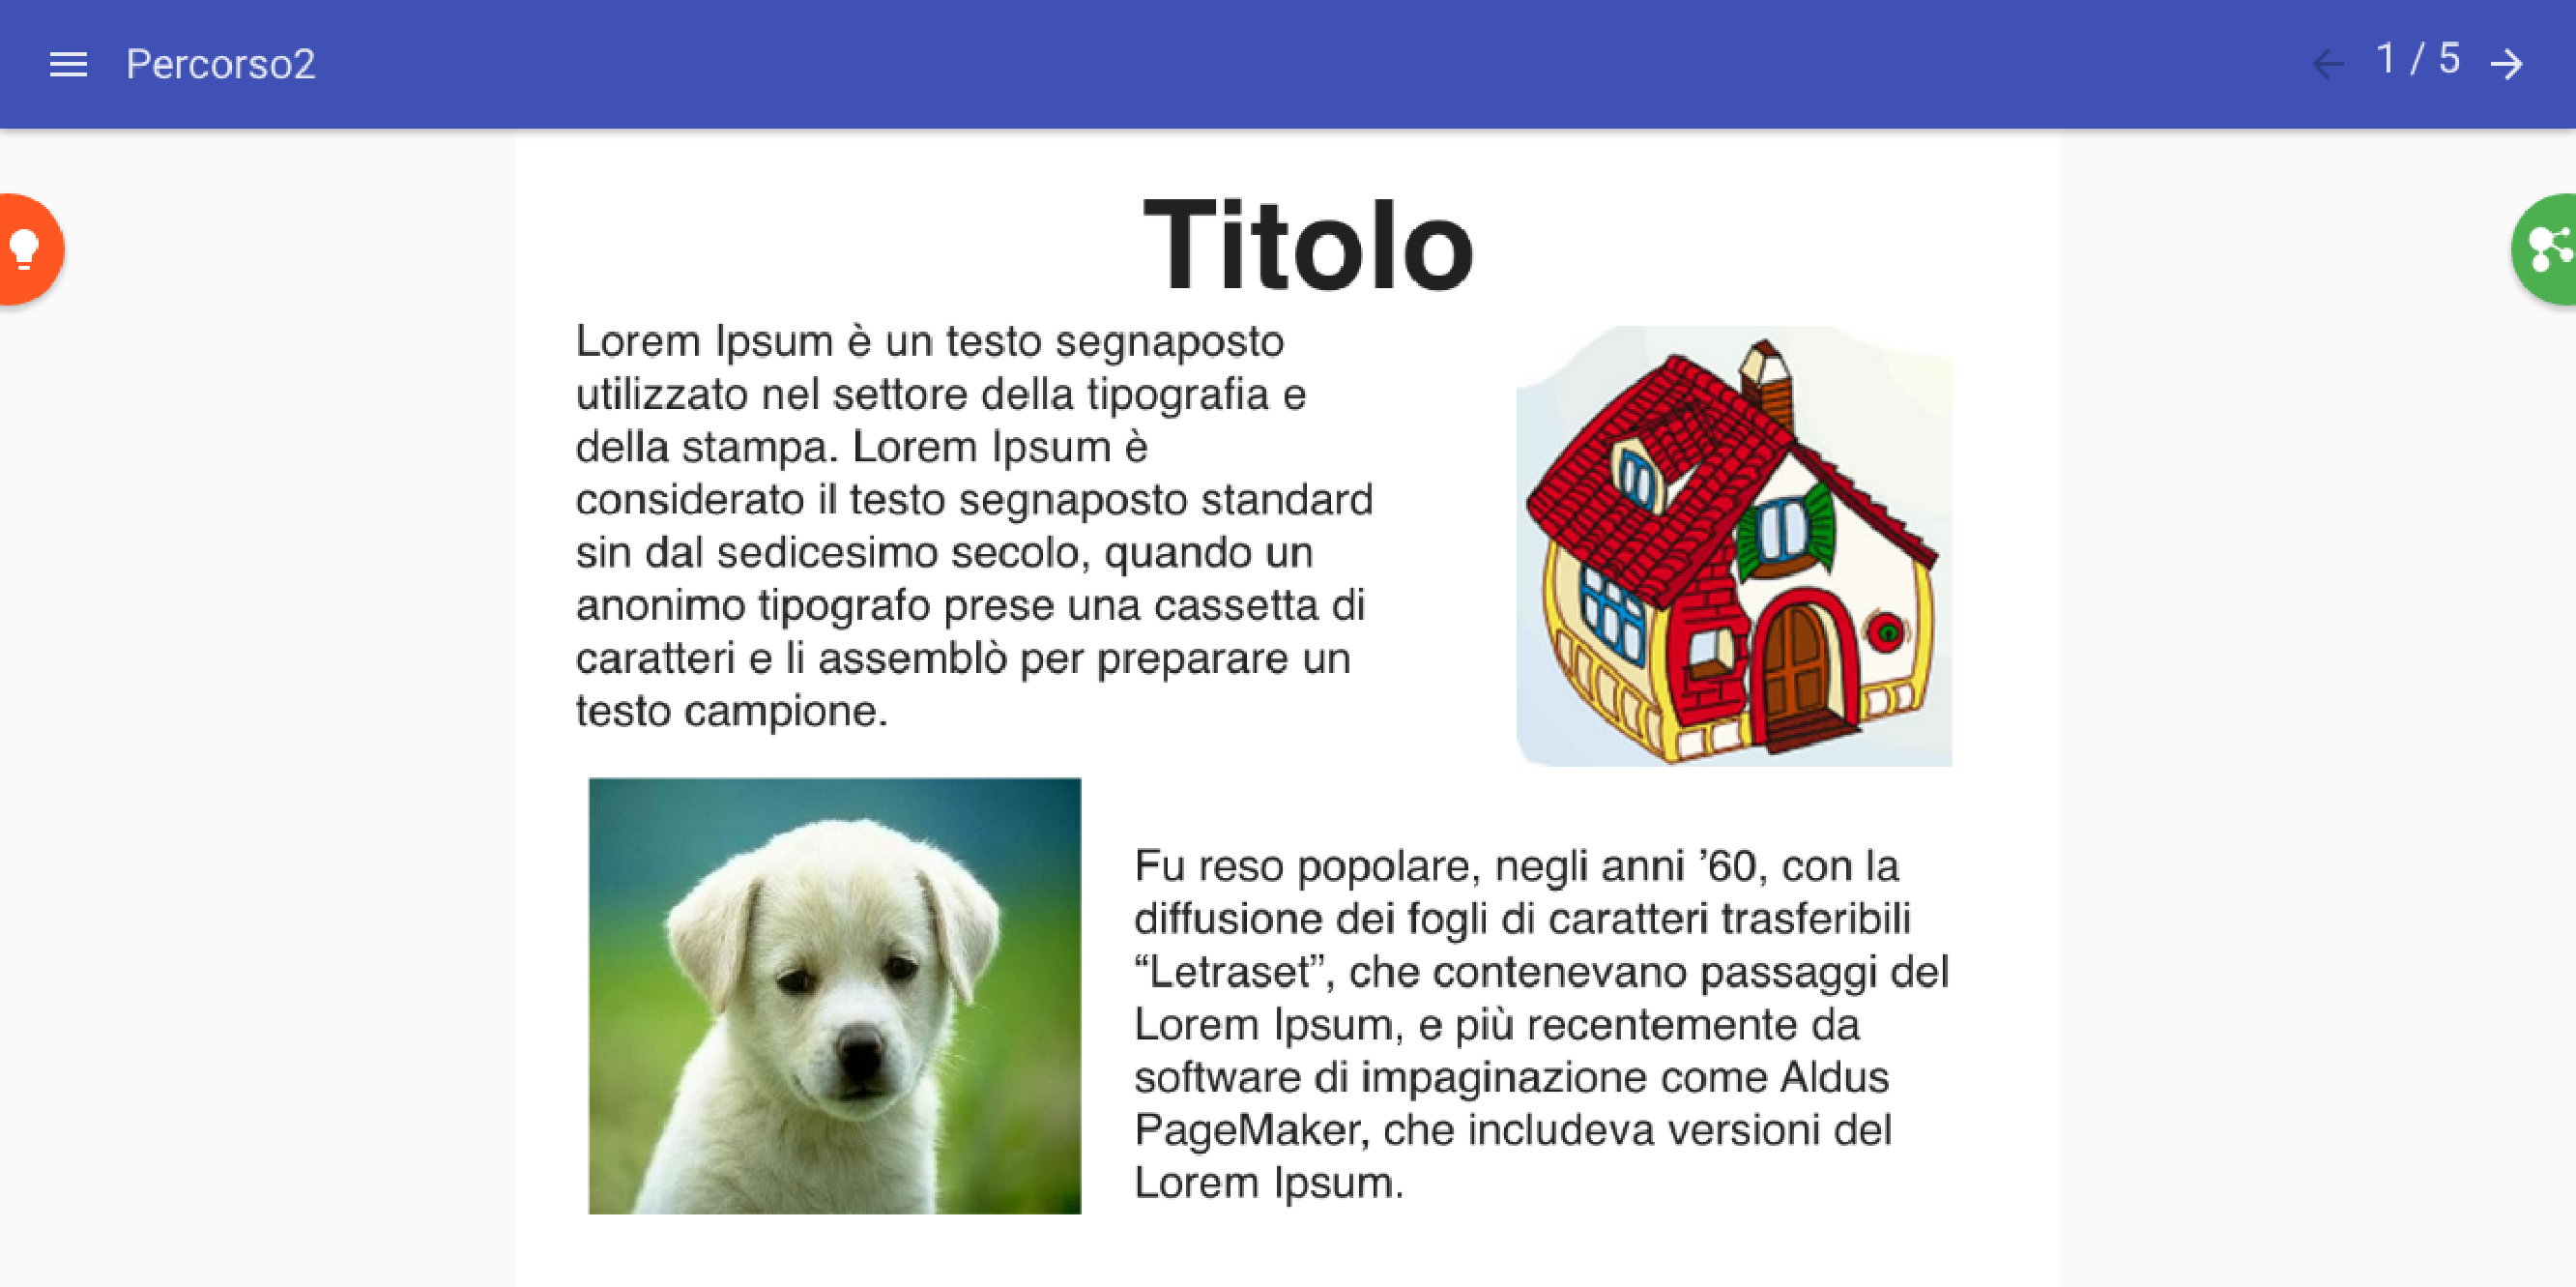
\includegraphics[scale=0.32]{immagini/presentazione.pdf}
\caption{Vista di presentazione}
\end{figure}
Questa pagina è dedicata all'esecuzione di presentazione, cioè la visualizzazione ordinata di una sequenza di \gloxy{frame}.\\
L'utente può accedere a questa pagina dopo aver selezionato un \gloxy{progetto}, scelto un \gloxy{percorso di presentazione} personalizzato e aver selezionato l'avvio della presentazione. \\
La presentazione viene generata utilizzando i \gloxy{frame} presenti all'interno dei nodi della mappa mentale, i quali verranno visualizzati secondo l'ordine stabilito dal \gloxy{percorso} di presentazione.
\subsection{Pannello di navigazione}
Gli strumenti principali che permette all'utente di spostarsi all'interno della presentazione sono \textbf{freccia a destra} 
\includegraphics[scale=0.5]{immagini/frecciaDestra.pdf} e \textbf{freccia a sinistra} 
\includegraphics[scale=0.5]{immagini/frecciaSinistra.pdf} che si trova in alto a destra nella vista di presentazione e i due menù laterali.
\begin{figure}[H]
\centering
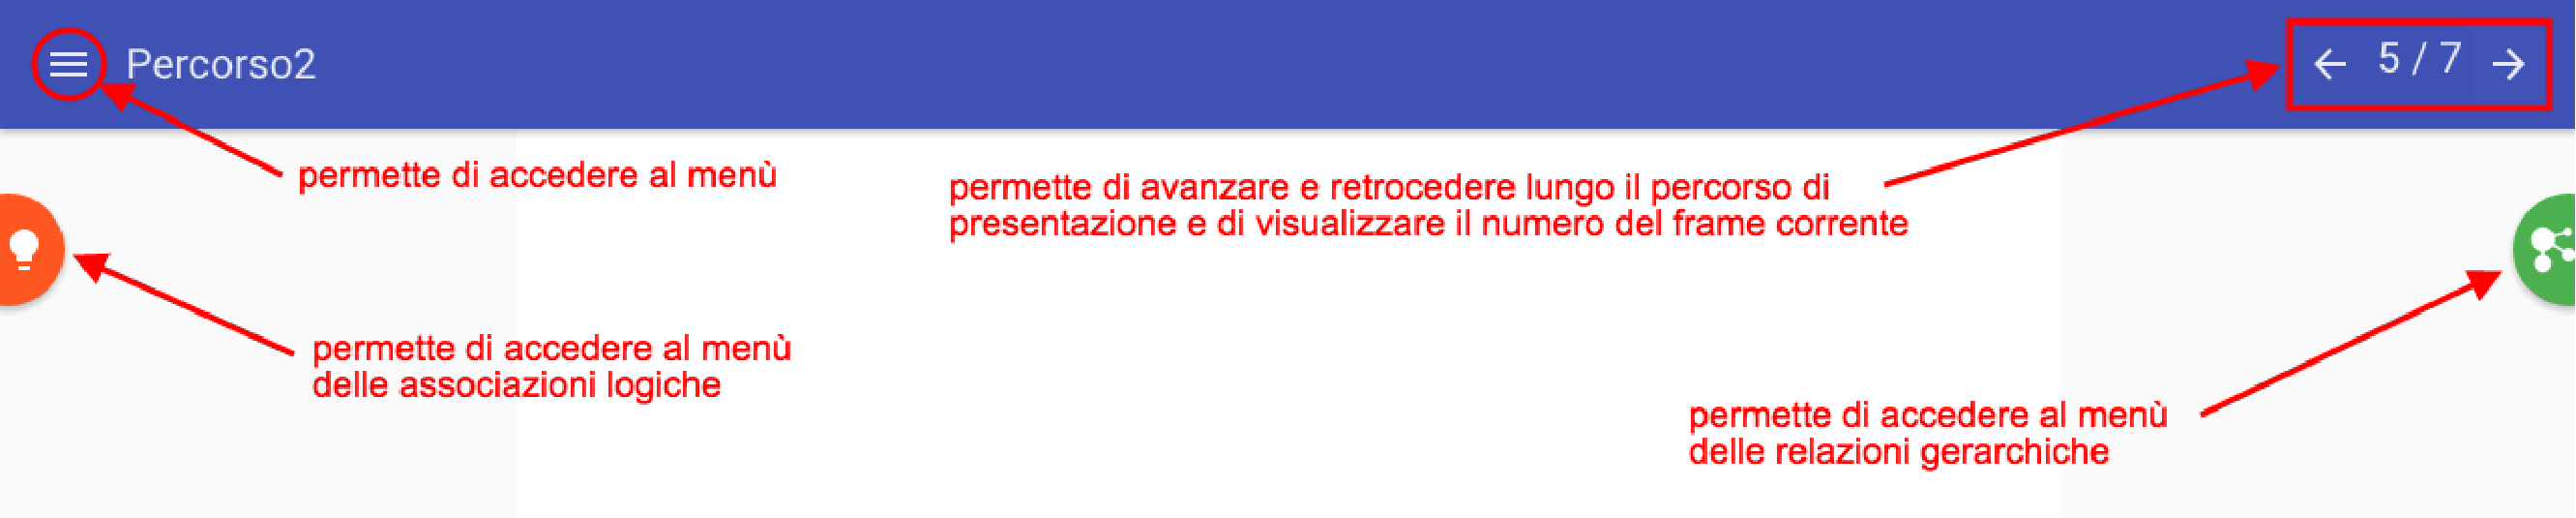
\includegraphics[scale=0.32]{immagini/imgFrecciePres.pdf}
\caption{Strumenti della vista di presentazione}
\end{figure}
\subsection{Menu laterali}
I due menu permettono all'utente di effettuare dei \textit{salti} dal \gloxy{frame} corrente ad un \gloxy{frame} ad esso correlato tramite relazione gerarchica o associazione logica.\\
Quando l'utente sta visualizzando un \textit{\gloxy{frame}} può passare alla visualizzazione di un altro \textit{\gloxy{frame}}, anche non appartenente al \gloxy{percorso} di presentazione, purché il nodo che lo contiene abbia un qualche tipo di relazione con quello corrente.
Una volta effettuato questo salto la presentazione passa in modalità ``\textit{non lineare}'', impedendo all'utente di cambiare \gloxy{frame} utilizzando le frecce.\\
Per riprendere la presentazione lineare e ritornare all'ultimo \gloxy{frame} del \gloxy{percorso} visualizzato è necessario premere l'apposito pulsante 
\includegraphics[scale=0.5]{immagini/frecciaRicurva.pdf} presente nel \textbf{\textit{Pannello di navigazione}}.
\subsubsection{Menu delle associazioni logiche}
\begin{figure}[H]
\centering
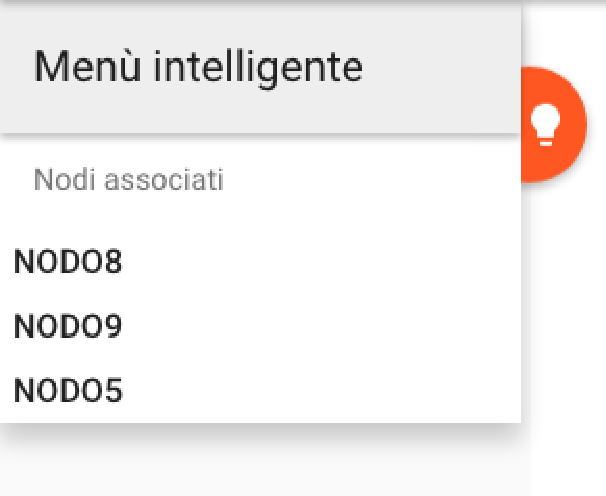
\includegraphics[scale=0.5]{immagini/menuLogico.pdf}
\caption{Menù delle associazioni logiche}
\end{figure}
Questo menu contiene una lista dei nodi della mappa mentale, collegati al nodo contenente il \gloxy{frame} corrente, tramite un'associazione logica.\\
L'utente può accedere a questo menù premendo l'etichetta a sinistra rappresentante una lampadina 
\includegraphics[scale=0.5]{immagini/lampadina.pdf}.\\
Selezionando uno dei nodi presenti all'interno di questo menu si andrà a visualizzare il \gloxy{frame} che contenuto in quel nodo, anche se il nodo non fa parte del \gloxy{percorso} di presentazione.
\subsubsection{Menu delle relazioni gerarchiche}
\begin{figure}[H]
\centering
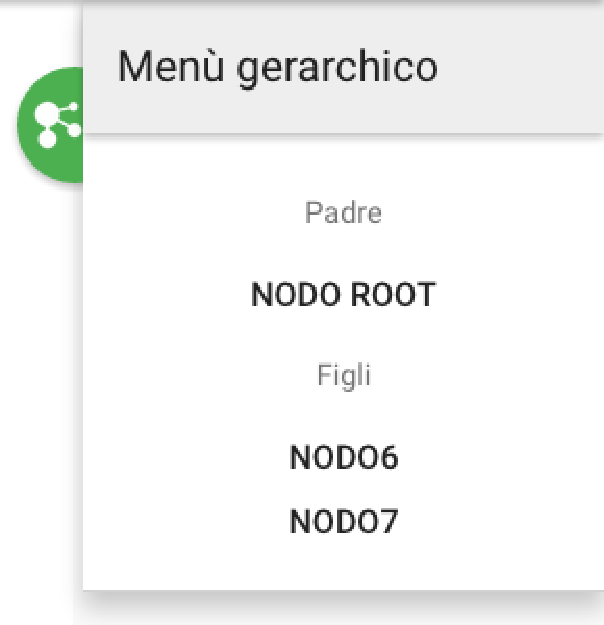
\includegraphics[scale=0.5]{immagini/menuGerarchico.pdf}
\caption{Menù delle relazioni gerarchiche}
\end{figure}
Questo menu contiene una lista dei nodi della mappa mentale, collegati al nodo contenente il \gloxy{frame} corrente tramite una relazione gerarchica.\\
L'utente può accedere a questo menù premendo l'etichetta a destra rappresentante un grafo 
\includegraphics[scale=0.5]{immagini/grafo.pdf} .\\
Selezionando uno dei nodi presenti all'interno di questo menu si andrà a visualizzare il \gloxy{frame} che rappresenta quel nodo, anche se il nodo non fa parte del \gloxy{percorso} di presentazione.

\section{Stampa di un progetto} \label{stamp}
L'applicazione \Premi offre la possibilità di effettuare la stampa in formato \gloxy{PDF}, su stampante e su iCloud\footnote{Funzionalità disponibile solo per i dispositivi Apple}, sia della \gloxy{mappa mentale} che della presentazione.\\
In seguito verranno descritti i procedimenti che consentono di eseguire le varie stampe.
\subsection{Stampa mappa mentale}
Per poter effettuare la stampa della mappa mentale, l'utente deve trovarsi nella pagina di modifica della \gloxy{mappa mentale} o in quella per la modifica dei \gloxy{percorsi} di presentazione.\\
Dovrà poi aprire il menù tramite il pulsante 
\includegraphics[scale=0.5]{immagini/buttonMenu.pdf} e selezionare la voce Stampa.\\
In seguito verrà visualizzata la finestra di stampa del \gloxy{browser} dalla quale sarà possibile selezionare le impostazioni di stampa, specificando se stampare come \gloxy{PDF} oppure stampare con una stampante.
Dal momento che viene stampata solamente la parte della \gloxy{mappa mentale} visualizzata a schermo, è consigliato regolare in modo opportuno lo \textit{zoom} della mappa, in modo da stamparla nella sua interezza.
\subsection{Stampa di una presentazione}\label{stampaPresentazione}
Per poter effettuare la stampa della presentazione, l'utente deve trovarsi nella pagina di \textit{presentazione}.\\
Dovrà poi aprire il menù tramite il pulsante 
\includegraphics[scale=0.5]{immagini/buttonMenu.pdf} e selezionare la voce Stampa.\\
In seguito verrà visualizzata la finestra di stampa del \gloxy{browser} dalla quale sarà possibile selezionare le impostazioni di stampa, specificando se stampare come \gloxy{PDF} oppure stampare con una stampante.

\section{Messaggi d'errore} \label{err}
Durante l'utilizzo dell'applicazione \Premi c'è la possibilità che si verifichino degli errori.\\
Questi vengono gestiti dall'applicazione fornendo all'utente un messaggio che lo informa sulla tipologia e sulla causa del malfunzionamento.\\
In seguito verranno elencati gli errori che possono essere sollevati dall'applicazione.
\subsection{Lista degli errori}
La lista che segue contiene il tipo di errore e la sua descrizione per gli errori specifici dell'applicazione \Premi.
\begin{itemize}
\item \texttt{Utente non trovato}: l'identificativo utente fornito non è un identificativo valido;
\item \texttt{Credenziali non valide}: è necessario fornire un indirizzo email ed una password valide;
\item \texttt{\gloxy{Progetto} non trovato}: l'identificativo del \gloxy{progetto} fornito non è un identificativo valido;
\item \texttt{Nodo non trovato}: l'identificativo del nodo fornito non è un identificativo valido;
\item \texttt{Associazione non trovata}: l'identificativo dell'associazione fornita non è un identificativo valido;
\item \texttt{\gloxy{Percorso} non trovato}: l'identificativo del \gloxy{percorso} fornito non è un identificativo valido;
\item \texttt{\gloxy{Progetto} corrotto}: errore nella ricerca dei campi dati relativi al \gloxy{progetto} indicato;
\item \texttt{Dati non validi}: i dati relativi al \gloxy{progetto} sono vuoti o errati;
\item \texttt{\gloxy{Progetto} corrotto}: errore durante l'eliminazione del \gloxy{progetto};
\item \texttt{Dati non validi}: i dati relativi al contenuto del nodo non sono validi o sono formattati in modo errato;
\item \texttt{Nodi non validi}: gli identificativi dei nodi forniti non sono validi oppure non esistono oppure il nodo entrante coincide con il nodo uscente;
\item \texttt{Dati non validi}: i dati per la modifica del \gloxy{percorso} non sono definiti;
\item \texttt{Nodo del \gloxy{progetto} non trovato}: il nodo riferito nella relazione o nel \gloxy{percorso} non è stato trovato all'interno del \gloxy{progetto} indicato;
\item \texttt{Nodo padre non esistente}: il nodo padre indicato non esiste o non corrisponde ad un nodo valido;
\item \texttt{Nodo non valido}: impossibile eliminare il nodo radice della mappa mentale.
\item \texttt{Nodo del \gloxy{percorso} non trovato}: il nodo riferito non è stato trovato all'interno del \gloxy{percorso} indicato.
\end{itemize}
Gli errori vengono segnalati all'utente tramite la visualizzazione di un \textit{popup}, in cui è presente la descrizione dell'errore.
\begin{figure}[H]
\centering

\includegraphics[scale=0.5]{immagini/errore.pdf}
\caption{Popup di notifica errore}
\end{figure}
Nel caso in cui l'utente desideri segnalare la presenza di errori non segnalati o ricevere informazioni specifiche riguardo agli errori dell'applicazione, può contattare il \gloxy{team} seguendo le indicazioni presenti nella sezione \textit{\nameref{sgnErr}}.

\section{Segnalazione degli errori} \label{sgnErr}
\subsection{Come segnalare dei bug o richiedere nuove funzionalità}
Se l'utente riscontrasse, durante l'utilizzo dell'applicazione \textbf{\textit{\progetto}}, eventuali \textit{bugs} o errori di altro genere o desiderasse richiedere l'aggiunta di nuove funzionalità che ritiene utili, può mandare una e-mail al team \textbf{\textit{\gruppo}} inserendo come oggetto il tipo di richiesta (es.:Segnalazione bug, Nuova funzionalità), e nel corpo una descrizione di essa.\\
L'indirizzo a cui sarà possibile inviare le segnalazioni è: \href{mailto:pragma.swe@gmail.com}{pragma.swe@gmail.com}
%glossario
\glsaddall
\ref{glossario}
\printglossary[title=Glossario]
\end{document}
